%%%%%%%%%%%%%%%%%%%%%%%%%%%%%%%%%%%%%%%%%%
% Mathematics Final Year Research Projects
% LaTeX Template
% Version 1.0 (31/01/24)
%
% This template has been adapted from: https://www.overleaf.com/latex/templates/imperial-college-report-template/wncnzptkhnbc
% Students should feel free to adapt this template to their needs.
%%%%%%%%%%%%%%%%%%%%%%%%%%%%%%%%%%%%%%%%%%
%----------------------------------------------------------------------------------------
% PACKAGES AND OTHER DOCUMENT CONFIGURATIONS
%----------------------------------------------------------------------------------------
\documentclass[a4paper,11pt, twoside]{report}

%% Language and font encodings
\usepackage[english]{babel}
\usepackage[utf8]{inputenc}
\usepackage[T1]{fontenc}

%% Imperial Recommended Packages
\usepackage{afterpage}

% Lean colour configurations
\usepackage{color}
\definecolor{keywordcolor}{rgb}{0.7, 0.1, 0.1}   % red
\definecolor{tacticcolor}{rgb}{0.0, 0.1, 0.6}    % blue
\definecolor{commentcolor}{rgb}{0.4, 0.4, 0.4}   % grey
\definecolor{symbolcolor}{rgb}{0.0, 0.1, 0.6}    % blue
\definecolor{sortcolor}{rgb}{0.1, 0.5, 0.1}      % green
\definecolor{attributecolor}{rgb}{0.7, 0.1, 0.1} % red
\definecolor{backcolour}{rgb}{0.95,0.95,0.92}

% Listings (for displaying code):
\usepackage{listings}
\def\lstlanguagefiles{TeX_Setup/lstlean.tex}
\lstset{
    % frame = single, 
    % framexleftmargin=15pt,
    language = lean,
    numbers = left,
    backgroundcolor=\color{backcolour}
}

% ----------- Algorithm2e setup
\usepackage[ruled,vlined]{algorithm2e}
\makeatletter
\renewcommand{\SetKwInOut}[2]{%
  \sbox\algocf@inoutbox{\KwSty{#2}\algocf@typo:}%
  \expandafter\ifx\csname InOutSizeDefined\endcsname\relax% if first time used
    \newcommand\InOutSizeDefined{}\setlength{\inoutsize}{\wd\algocf@inoutbox}%
    \sbox\algocf@inoutbox{\parbox[t]{\inoutsize}{\KwSty{#2}\algocf@typo:\hfill}~}\setlength{\inoutindent}{\wd\algocf@inoutbox}%
  \else% else keep the larger dimension
    \ifdim\wd\algocf@inoutbox>\inoutsize%
    \setlength{\inoutsize}{\wd\algocf@inoutbox}%
    \sbox\algocf@inoutbox{\parbox[t]{\inoutsize}{\KwSty{#2}\algocf@typo:\hfill}~}\setlength{\inoutindent}{\wd\algocf@inoutbox}%
    \fi%
  \fi% the dimension of the box is now defined.
  \algocf@newcommand{#1}[1]{%
    \ifthenelse{\boolean{algocf@inoutnumbered}}{\relax}{\everypar={\relax}}%
%     {\let\\\algocf@newinout\hangindent=\wd\algocf@inoutbox\hangafter=1\parbox[t]{\inoutsize}{\KwSty{#2}\algocf@typo\hfill:}~##1\par}%
    {\let\\\algocf@newinout\hangindent=\inoutindent\hangafter=1\parbox[t]{\inoutsize}{\KwSty{#2}\algocf@typo:\hfill}~##1\par}%
    \algocf@linesnumbered% reset the numbering of the lines
  }}%
\makeatother
% --------- end algorithm2e setup

\usepackage{bm}
\usepackage[normalem]{ulem}

\usepackage[colorinlistoftodos]{todonotes}

% I have all of their other recommended packages somewhere on here.

\usepackage[most]{tcolorbox}
\usepackage{authblk}  % Lets you add an \affil{} to your title, stating your affiliation {eg. Sigma Mathematics Society}
\usepackage{ragged2e}
\usepackage{csquotes}
\usepackage{pdfpages}



\usepackage{xfrac}
\usepackage{cancel}

\usepackage[inline]{enumitem}

%\usepackage{tgpagella}

\usepackage{blindtext}
\usepackage{lipsum}
\usepackage{verbatim}
\usepackage{hyperref}
\hypersetup{
    citebordercolor = 1 1 1,
    linkbordercolor = 1 1 1,
    filebordercolor = 1 1 1,
    menubordercolor = 1 1 1,
    urlbordercolor = 1 1 1,
    colorlinks  =   true,
    linkcolor   =   blue,
    citecolor   =   magenta,
    urlcolor    =   blue
}

% This project uses natbib instead. See end of format file.
% \usepackage{biblatex} % Modify citation format using [style=yourstyle] parameter--eg \usepackage[style=mla-new]{biblatex}
% \bibliography{TeX_Setup/References.bib}
% \addbibresource{TeX_Setup/References.bib}

\usepackage{cancel}
\usepackage{amssymb}
\usepackage{amsmath}
% \usepackage{amsthm}  % In `environments.tex`
%\usepackage{MnSymbol}
\usepackage{mathrsfs}
\usepackage{mathtools}
% \usepackage{mathabx}
\usepackage{mathdots}
\usepackage{yhmath}

\usepackage{array}
\usepackage{booktabs}
\usepackage{longtable}

\usepackage{graphicx}
\newcommand\sbullet[1][.5]{\mathbin{\vcenter{\hbox{\scalebox{#1}{$\bullet$}}}}}  % Bullet of customisable size
\usepackage{wrapfig}
% Imperial-recommended `caption` setup
\usepackage{caption}
\captionsetup[figure]{labelfont={bf}, name={Figure}, justification=centering}
\captionsetup[table]{labelfont={bf}, name={Table}}
\usepackage{subcaption}
\usepackage{tikz}
\usepackage{float}

% Tikz
\usepackage{tikz-cd}
\usepackage{tikz-3dplot}
\usetikzlibrary{positioning}
\usetikzlibrary{cd}
\usetikzlibrary{shapes.geometric}
\usepackage{pgfplots}
\usepackage{mathrsfs}
\usetikzlibrary{arrows}
\usepackage{qtree}

%% Sets page size and margins
\usepackage[a4paper,top=1in,bottom=1in,left=1in,right=1in,marginparwidth=1.75cm]{geometry}

% Font

% \usepackage{sansmathfonts}
% % \usepackage{mathrsfs}
% \usepackage[T1]{fontenc}
% \renewcommand*\familydefault{\sfdefault}

\renewcommand*{\rmdefault}{bch}
\renewcommand*{\ttdefault}{lmtt}

% Structure and Numbering

\usepackage{fancyhdr}
\usepackage{lastpage}

\pagestyle{fancy}
\fancyhf{}

\rhead{{Page \thepage}}%\hspace{1pt} of \pageref{LastPage}}}
\lhead{\textit\slshape\nouppercase{\leftmark}}

\numberwithin{equation}{section}

% Lists

\setlist[description]{font=\normalfont}
\setlist[enumerate]{before=\normalfont}

% Spacing and indentation

% Not sure if 1.5-spacing is permitted. I'll leave it commented out for now.
% \usepackage{setspace}
% \renewcommand{\baselinestretch}{1.5}

\usepackage[skip=11pt, indent=0pt]{parskip}
% Here's what Imperial's recommended setup is:
% \setlength{\parskip}{0.5em}
% \usepackage{indentfirst}  % Uncomment if using above

\allowdisplaybreaks  % Allows align environments to continue for several pages

% Colours

\usepackage{xcolor}
\definecolor{darkblue}{rgb}{0.0, 0.0, 0.55}
\definecolor{pink}{rgb}{0.858, 0.188, 0.478}
\definecolor{brown}{rgb}{0.8, 0.4, 0.0}

% Bibliography
\usepackage[numbers, comma, square, sort&compress]{natbib}
\bibliographystyle{References/abbrvunsrtnat.bst}
% \bibliographystyle{unsrtnat}

\usepackage{amsthm}
% Gives theorem and definition names the same font style as the words "theorem"/"definition": see https://tex.stackexchange.com/questions/43966/how-to-make-the-optional-title-of-a-theorem-bold-with-amsthm
\makeatletter
\def\th@plain{%
  \thm@notefont{}% same as heading font
  \itshape % body font
}
\def\th@definition{%
  \thm@notefont{}% same as heading font
  \normalfont % body font
}
\makeatother

\usepackage{cleveref}

\newtheorem*{theorem*}{Theorem}
\newtheorem{theorem}{Theorem}[section]
\newtheorem{corollary}[theorem]{Corollary}%[theorem]
\newtheorem{lemma}[theorem]{Lemma}
\newtheorem{claim}[theorem]{Claim}
\newtheorem{conjecture}[theorem]{Conjecture}
% \newtheorem{algorithm}[theorem]{Algorithm}  % Defined in algorithm2e
\newtheorem{proposition}[theorem]{Proposition}

\newtheorem{problem}[theorem]{Problem}
\newenvironment{boxproblem}{
    \begin{tcolorbox}[colback=yellow!15!white,colframe=orange, breakable, enhanced]\begin{problem}
}{
    \end{problem}\end{tcolorbox}
}

\newenvironment{boxtheorem}{
    \begin{tcolorbox}[colback=yellow!15!white,colframe=orange, breakable, enhanced]\begin{theorem}
}{
    \end{theorem}\end{tcolorbox}
}
\newenvironment{boxproposition}{
    \begin{tcolorbox}[colback=yellow!15!white,colframe=orange, breakable, enhanced]\begin{proposition}
}{
    \end{proposition}\end{tcolorbox}
}
\newenvironment{boxlemma}{
    \begin{tcolorbox}[colback=yellow!15!white,colframe=orange, breakable, enhanced]\begin{lemma}
}{
    \end{lemma}\end{tcolorbox}
}
\newenvironment{boxcorollary}{
    \begin{tcolorbox}[colback=yellow!15!white,colframe=orange, breakable, enhanced]\begin{corollary}
}{
    \end{corollary}\end{tcolorbox}
}
\newenvironment{boxconjecture}{
    \begin{tcolorbox}[colback=yellow!15!white,colframe=orange, breakable, enhanced]\begin{conjecture}
}{
    \end{conjecture}\end{tcolorbox}
}


\theoremstyle{remark}
\newtheorem*{remark}{Remark}
\newtheorem*{solution}{Solution}

\theoremstyle{definition}
\newtheorem{definition}[theorem]{Definition}
\newenvironment{boxdefinition}{
    \begin{tcolorbox}[colback=cyan!10!white,colframe=cyan!70!black, breakable, enhanced]\begin{definition}
}{
    \end{definition}\end{tcolorbox}
}
\newtheorem*{convention}{Convention}
\newenvironment{boxconvention}{
    \begin{tcolorbox}[colback=magenta!3!white,colframe=magenta!70!black, breakable, enhanced]\begin{convention}
}{
    \end{convention}\end{tcolorbox}
}
\newtheorem*{notation}{Notation}
\newenvironment{boxnotation}{
    \begin{tcolorbox}[colback=magenta!3!white,colframe=magenta!70!black, breakable, enhanced]\begin{notation}
}{
    \end{notation}\end{tcolorbox}
}
\newtheorem{example}[theorem]{Example}
\newenvironment{boxexample}{
    \begin{tcolorbox}[colframe=green!30!black, breakable, enhanced, breakable, enhanced]\begin{example}
}{
    \end{example}\end{tcolorbox}
}
\newtheorem{nexample}[theorem]{Non-Example}
\newenvironment{boxnexample}{
    \begin{tcolorbox}[colframe=red!50!black, breakable, enhanced]\begin{nexample}
}{
    \end{nexample}\end{tcolorbox}
}
\newtheorem{cexample}[theorem]{Counterexample}
\newenvironment{boxcexample}{
    \begin{tcolorbox}[colframe=red!50!black, breakable, enhanced]\begin{cexample}
}{
    \end{cexample}\end{tcolorbox}
}

% \def\SMALLCOLWIDTH{1.5cm}
\newcolumntype{C}[1]{>{\centering\let\newline\\\arraybackslash\hspace{0pt}}m{#1}}

% Centering captions
% \renewcommand{\caption}[1]{\caption{\centering #1}}

%%%%%%%%%%%%%%%%%%%%%%%%%%%%%%%%%%%%%%%%%%%%%%%%%%%%%%%%%%%%%%%%%%%%%%%%%%%%%%%%%%%%%%%%%%%%%%%%%%%%%%%%%%%%
% CUSTOM COMMANDS
%%%%%%%%%%%%%%%%%%%%%%%%%%%%%%%%%%%%%%%%%%%%%%%%%%%%%%%%%%%%%%%%%%%%%%%%%%%%%%%%%%%%%%%%%%%%%%%%%%%%%%%%%%%%

% Custom colours

\definecolor{darkgreen}{rgb}{0.1, 0.4, 0.3}      % green

% `sorry`

\newcommand{\sorry}{\textcolor{red}{\texttt{sorry}}}
% \newcommand{\sorry}{\lstinline{sorry}}

% TIKZ:

\newcommand{\drawplane}{  % For use with TikZ
    \draw[step=0.5cm,gray,very thin] (-2.5,-2.5) grid (2.5,2.5);
    \draw[thick,->] (-2.5,0) -- (2.5,0); % node[anchor=west] {$x$};
    \draw[thick,->] (0,-2.5) -- (0,2.5); % node[anchor=south] {$y$};
    % \node[black, anchor=north east] at (0, 0) {$0$};
}
\newcommand{\latticecircle}[2]{
    \draw[fill=yellow, opacity=0.5] (#1, #2) circle (0.5);
    \node at (#1, #2) {\color{gray}{$\bullet$}};
}
\newcommand{\latticecirclegrey}[2]{
    \draw[fill=gray, opacity=0.75] (#1, #2) circle (0.5);
    \node at (#1, #2) {\color{black}{$\bullet$}};
}
\newcommand{\latticecirclebrown}[2]{
    \draw[fill=brown, opacity=0.75] (#1, #2) circle (0.5);
    \node at (#1, #2) {\color{black}{$\bullet$}};
}
\usetikzlibrary{decorations.markings}
\tikzset{->-/.style={decoration={
      markings,
      mark=at position #1 with {\arrow{>}}},postaction={decorate}
}}

\newenvironment{cd}{
    \begin{equation} \begin{tikzcd}
}{
    \end{tikzcd} \end{equation}
}
\newenvironment{cd*}{
    \begin{equation*} \begin{tikzcd}
}{
    \end{tikzcd} \end{equation*}
}

\newcommand{\drawsquare}[1]{
    \draw[thick, blue]
    (-{#1},-{#1}) node [anchor=north east] {C} --
    (-{#1}, {#1}) node[anchor=south east] {B} --
    ({#1}, {#1}) node[anchor=south west] {A} --
    ({#1}, -{#1}) node [anchor=north west] {D} -- cycle;
}

\newcommand{\labelledpoint}[5]{ % Takes x coord, y coord, label x-position relative to point, label y-position relative to point, label text as arguments
    \node [label={[shift={(#3,#4)}]#5}] at (#1, #2) {$\bullet$};
}

% DELIMITERS:

\newcommand{\parenth}[1]{\left( #1 \right)}
\newcommand{\brac}[1]{\left[ #1 \right]}
\newcommand{\set}[1]{\left\{ #1 \right\}}
\newcommand{\setst}[2]{\set{#1 \; \middle\vert \; #2}}
\newcommand{\abs}[1]{\left\lvert #1 \right\rvert}
\newcommand{\norm}[1]{\left\lVert #1 \right\rVert}
\newcommand{\floor}[1]{\left\lfloor #1 \right\rfloor}
\newcommand{\ceil}[1]{\left\lceil #1 \right\rceil}
\newcommand{\cycl}[1]{\left\langle #1 \right\rangle}
\newcommand{\grpres}[2]{\cycl{#1 \; \middle| \; #2}}  % \grpres{gens}{rels}

% FUNCTIONS:

\newcommand{\fx}{f\!\parenth{x}}
\newcommand{\fof}[1]{f\!\parenth{#1}}

\newcommand{\px}{p\!\parenth{x}}
\newcommand{\pof}[1]{p\!\parenth{#1}}
\newcommand{\pofbig}[1]{p\Big(#1\Big)}
\newcommand{\gx}{g\!\parenth{x}}
\newcommand{\gof}[1]{g\!\parenth{#1}}
\newcommand{\hx}{h\!\parenth{x}}
\newcommand{\hof}[1]{h\!\parenth{#1}}
\newcommand{\Tv}{T\!\parenth{v}}
\newcommand{\Tof}[1]{T\!\parenth{#1}}
\newcommand{\Tbar}{\overline{T}}
\newcommand{\Tbarof}[1]{\Tbar\!\parenth{#1}}
\newcommand{\Tbarv}{\Tbarof{v}}
\newcommand{\Sof}[1]{S\!\parenth{#1}}

\newcommand{\psin}[1]{\sin\!{\parenth{#1}}}
\newcommand{\pcos}[1]{\cos\!{\parenth{#1}}}
\newcommand{\ptan}[1]{\tan\!{\parenth{#1}}}
\newcommand{\sinsq}[1]{\sin^2\!\parenth{#1}}
\newcommand{\cossq}[1]{\cos^2\!\parenth{#1}}
\newcommand{\tansq}[1]{\tan^2\!\parenth{#1}}
\newcommand{\parcsin}[1]{\arcsin\!{\parenth{#1}}}
\newcommand{\parccos}[1]{\arccos\!{\parenth{#1}}}
\newcommand{\parctan}[1]{\arctan\!{\parenth{#1}}}

\newcommand{\logbase}[2]{\log_{#1}\!\parenth{#2}}
\newcommand{\nthroot}[2]{\sqrt[\leftroot{-3}\uproot{3} #1]{#2}}
\newcommand{\cbrt}[1]{\nthroot{3}{#1}}

\newcommand{\pgcd}[2]{\gcd\!\parenth{{#1},{#2}}}
\newcommand{\plcm}[2]{\operatorname{lcm}\!\parenth{{#1},{#2}}}
\newcommand{\pgcds}[1]{\gcd\!\parenth{#1}}
\newcommand{\plcms}[1]{\operatorname{lcm}\!\parenth{#1}}

\newcommand{\varphiof}[1]{\varphi\!\parenth{#1}}
\newcommand{\phiof}[1]{\phi\!\parenth{#1}}
\newcommand{\xiof}[1]{\xi\!\parenth{#1}}
\newcommand{\rhoof}[1]{\rho\!\parenth{#1}}
\newcommand{\pexp}[1]{\exp\!\parenth{#1}}

\newcommand{\inj}{\hookrightarrow}
\newcommand{\surj}{\twoheadrightarrow}

\DeclareMathOperator*{\argmin}{\arg\!\min}
\DeclareMathOperator*{\argmax}{\arg\!\max}

\newcommand{\of}[1]{\!\parenth{#1}}

% CALCULUS:

\newcommand{\dx}{\operatorname{d}\!x}
\newcommand{\dy}{\operatorname{d}\!y}
\newcommand{\diff}[1]{\operatorname{d}\!{#1}}
\newcommand{\dydx}{\frac{\dy}{\dx}}

% LINEAR ALGEBRA:

\newcommand{\mat}[3]{\operatorname{M}_{{#1} \times {#2}}\!\parenth{{#3}}}
\newcommand{\matsq}[2]{\operatorname{M}_{{#1} \times {#1}}\!\parenth{\mathbb{#2}}}
\newcommand{\MnR}{\operatorname{M}_{n}\!\parenth{\real}}
\newcommand{\MnC}{\operatorname{M}_{n}\!\parenth{\C}}
\newcommand{\Mn}[2]{\operatorname{M}_{#1}\!\parenth{#2}}
\newcommand{\GL}[1]{\operatorname{GL}\!\parenth{#1}}
\newcommand{\SL}[1]{\operatorname{SL}\!\parenth{#1}}
\newcommand{\PGL}[1]{\operatorname{PGL}\!\parenth{#1}}
\newcommand{\PSL}[1]{\operatorname{PSL}\!\parenth{#1}}

\newcommand{\Span}[1]{\operatorname{Span}\!\parenth{#1}}

\newcommand{\pdim}[1]{\dim\!\parenth{#1}}

\newcommand{\RSp}[1]{\operatorname{RSp}\!\parenth{#1}}
\newcommand{\CSp}[1]{\operatorname{CSp}\!\parenth{#1}}
\newcommand{\rank}[1]{\operatorname{rank}\!\parenth{#1}}
\newcommand{\pim}[1]{\operatorname{im}\!\parenth{#1}}
\newcommand{\pker}[1]{\operatorname{ker}\!\parenth{#1}}
\newcommand{\pdet}[1]{\det\!\parenth{#1}}

\newcommand{\cA}[1]{c_A \! \parenth{#1}}
\newcommand{\cB}[1]{c_B \! \parenth{#1}}
\newcommand{\mA}[1]{m_A \! \parenth{#1}}
\newcommand{\mB}[1]{m_B \! \parenth{#1}}
\newcommand{\cAx}{\cA{x}}
\newcommand{\cBx}{\cB{x}}
\newcommand{\mAx}{\mA{x}}
\newcommand{\mBx}{\mB{x}}
\newcommand{\cof}[2]{c_{#1}\!\parenth{#2}}
\newcommand{\mof}[2]{m_{#1}\!\parenth{#2}}

\newcommand{\Cof}[1]{C\!\parenth{#1}}
\newcommand{\+}{\oplus}
\newcommand{\pdeg}[1]{\deg\!\parenth{#1}}

\newcommand{\RCF}[1]{\operatorname{RCF}\!\parenth{#1}}
\newcommand{\JCF}[1]{\operatorname{JCF}\!\parenth{#1}}

\newcommand{\Jsub}[2]{J_{#1}\!\parenth{#2}}

\newcommand{\Aof}[1]{A\!\parenth{#1}}

\newcommand{\Tsub}[2]{T_{#1}\!\parenth{#2}}

\newcommand{\Tr}[1]{\operatorname{Tr}\!\parenth{#1}}

\newcommand{\diag}[1]{\operatorname{diag}\!\parenth{#1}}

% Measure Theory

\newcommand{\muof}[1]{\mu\!\parenth{#1}}
\newcommand{\muA}{\muof{A}}
\newcommand{\muB}{\muof{B}}
\newcommand{\mutof}[1]{\Tilde{\mu}\!\parenth{#1}}
\newcommand{\mustof}[1]{\mu^*\!\parenth{#1}}
\newcommand{\calF}{\mathcal{F}}
\newcommand{\calA}{\mathcal{A}}
\newcommand{\calB}{\mathcal{B}}
\newcommand{\calC}{\mathcal{C}}
\newcommand{\sigmaof}[1]{\sigma\!\parenth{#1}}
\newcommand{\psiof}[1]{\psi\!\parenth{#1}}

% Intervals

\newcommand{\Ioc}[1]{\left(#1\right]}
\newcommand{\Ico}[1]{\left[#1\right)}

% GROUPS/ALGEBRA IN GENERAL:

\newcommand{\inv}{^{-1}}
\newcommand{\Sym}[1]{\operatorname{Sym}\!\parenth{#1}}
\newcommand{\ord}[1]{\operatorname{ord}\!\parenth{#1}}
\newcommand{\supp}[1]{\operatorname{supp}\!\parenth{#1}}
\newcommand{\sgn}[1]{\operatorname{sgn}\!\parenth{#1}}
\newcommand{\tcyc}[2]{\begin{pmatrix} #1 & #2 \end{pmatrix}}

\newcommand{\nsg}{\trianglelefteq}

\newcommand{\Rmul}{R^{\times}}
\newcommand{\kmul}{k^{\times}}
\newcommand{\kX}{k\!\brac{X}}
\newcommand{\RX}{R\!\brac{X}}

\newcommand{\quotient}[2]{
    \left.\raisebox{.2em}{${#1}$} \middle/ \raisebox{-.2em}{${#2}$} \right.
}
\newcommand{\Zmod}[1]{\quotient{\Z}{{#1}\Z}}

\newcommand{\Vof}[1]{V\!\parenth{#1}}

\newcommand{\Frac}[1]{\operatorname{Frac}\!\parenth{#1}}

\newcommand{\Spec}[1]{\operatorname{Spec}\!\parenth{#1}}

\newcommand{\id}{\operatorname{id}}

\newcommand{\pchar}[1]{\operatorname{char}\!\parenth{#1}}

\newcommand{\Hom}{\operatorname{Hom}}

\newcommand{\Zof}[1]{\operatorname{Z}\!\parenth{#1}}

\newcommand{\Aut}[1]{\operatorname{Aut}\!\parenth{#1}}

% NUMBER SETS:

\newcommand{\real}{\mathbb{R}}
\newcommand{\rational}{\mathbb{Q}}
\newcommand{\naturalnum}{\mathbb{N}}
\newcommand{\integers}{\mathbb{Z}}
\newcommand{\complex}{\mathbb{C}}

\newcommand{\Field}{\mathbb{F}}
\newcommand{\Q}{\mathbb{Q}}
\newcommand{\R}{\real}
\newcommand{\N}{\naturalnum}
\newcommand{\Z}{\integers}
\newcommand{\C}{\complex}
\newcommand{\B}{\mathcal{B}}
\newcommand{\I}{\mathcal{I}}
\newcommand{\J}{\mathcal{J}}

\newcommand{\psup}[1]{\sup\!\parenth{#1}}
\newcommand{\pinf}[1]{\inf\!\parenth{#1}}

% LOGIC:

\newcommand{\ergo}{\therefore}
\newcommand{\bcos}{\because}
\newcommand{\st}{\text{ s.t. }}


% -------------------- SPECIFIC TO PROJECT -------------------- %

% TERMINOLOGY

\newcommand{\CELP}{Cohn-Elkies Linear Programming Bound}
\newcommand{\CEC}{Cohn-Elkies Conditions}
\newcommand{\JCT}{Jordan Curve Theorem}
\newcommand{\CGT}{Cauchy-Goursat Theorem}

% NOTATION

\newcommand{\Pa}{\mathcal{P}}
\newcommand{\Vol}{\operatorname{Vol}}
\newcommand{\Volof}[1]{\Vol\!\parenth{#1}}
\newcommand{\Sch}{\mathcal{S}}
\renewcommand{\hat}{\widehat}
\renewcommand{\tilde}{\widetilde}
\newcommand{\F}{\mathcal{F}}
\newcommand{\periodic}{\operatorname{periodic}}

\newcommand{\Halfplane}{\mathbb{H}} % Using Lean notation for the upper-half plane instead of Viazovska's

\newcommand{\BigO}[1]{\operatorname{O}\of{#1}}

\newcommand{\fm}{f \mid}
\newcommand{\fmof}[3]{\parenth{\fm_{#1} {#2}}\of{#3}}

% COMPLEX ANALYSIS

\renewcommand{\Re}{\operatorname{Re}}
\renewcommand{\Im}{\operatorname{Im}}

\newcommand{\rad}{_{\operatorname{rad}}}

% LEAN

\newcommand{\mathlib}{\texttt{mathlib}}


% %% Useful packages
% \usepackage{afterpage}
% \usepackage{amsmath}
% \usepackage{amsthm}
% \usepackage{amssymb}
% \usepackage{csquotes}
% \usepackage{enumitem}
% \usepackage{graphicx}
% \usepackage{lipsum}
% \usepackage{booktabs}

% % Listings (for displaying code):
% \usepackage{listings}
% \lstset{
%     frame = single, 
%     framexleftmargin=15pt
% }

% % Center figure captions:
% \usepackage{caption}
% \captionsetup[figure]{labelfont={bf},name={Figure},labelsep=quad}
% \captionsetup[table]{labelfont={bf},name={Table},labelsep=quad}


% % ----------- Algorithm2e setup
% \usepackage[ruled,vlined]{algorithm2e}
% \makeatletter
% \renewcommand{\SetKwInOut}[2]{%
%   \sbox\algocf@inoutbox{\KwSty{#2}\algocf@typo:}%
%   \expandafter\ifx\csname InOutSizeDefined\endcsname\relax% if first time used
%     \newcommand\InOutSizeDefined{}\setlength{\inoutsize}{\wd\algocf@inoutbox}%
%     \sbox\algocf@inoutbox{\parbox[t]{\inoutsize}{\KwSty{#2}\algocf@typo:\hfill}~}\setlength{\inoutindent}{\wd\algocf@inoutbox}%
%   \else% else keep the larger dimension
%     \ifdim\wd\algocf@inoutbox>\inoutsize%
%     \setlength{\inoutsize}{\wd\algocf@inoutbox}%
%     \sbox\algocf@inoutbox{\parbox[t]{\inoutsize}{\KwSty{#2}\algocf@typo:\hfill}~}\setlength{\inoutindent}{\wd\algocf@inoutbox}%
%     \fi%
%   \fi% the dimension of the box is now defined.
%   \algocf@newcommand{#1}[1]{%
%     \ifthenelse{\boolean{algocf@inoutnumbered}}{\relax}{\everypar={\relax}}%
% %     {\let\\\algocf@newinout\hangindent=\wd\algocf@inoutbox\hangafter=1\parbox[t]{\inoutsize}{\KwSty{#2}\algocf@typo\hfill:}~##1\par}%
%     {\let\\\algocf@newinout\hangindent=\inoutindent\hangafter=1\parbox[t]{\inoutsize}{\KwSty{#2}\algocf@typo:\hfill}~##1\par}%
%     \algocf@linesnumbered% reset the numbering of the lines
%   }}%
% \makeatother
% % --------- end algorithm2e setup

% % \bm allows typing bold math:
% \usepackage{bm}
% \usepackage[normalem]{ulem}

% \usepackage[colorinlistoftodos]{todonotes}
% \usepackage[colorlinks=true, allcolors=blue]{hyperref}

% \renewcommand*{\rmdefault}{bch}
% \renewcommand*{\ttdefault}{lmtt}
% \newcommand{\citationneeded}{\textcolor{red}{[citation-needed]}}

% % Add bigger skip between paragraphs, makes reading easier:
% \setlength{\parskip}{0.5em}

% % Bibliography
% \usepackage[numbers, comma, square, sort&compress]{natbib}
% \bibliographystyle{References/abbrvunsrtnat.bst}

%----------------------------------------------------------------------------------------
% END OF DOCUMENT CONFIGURATION
%----------------------------------------------------------------------------------------

%----------------------------------------------------------------------------------------
% IMPORTANT INFORMATION TO MODIFY FOR THE TITLE PAGE
%----------------------------------------------------------------------------------------
\newcommand{\reporttitle}{Viazovska's Magic Function in Dimension 8: \\ A Formalisation in Lean} % Title of your research project
\newcommand{\reportauthor}{Sidharth Hariharan} % First Name and Last Name
\newcommand{\supervisor}{Bhavik Mehta} % First Name and Last Name of your supervisor(s)
\newcommand{\degreetype}{MSci in Mathematics} % MSci in Mathematics, BSc in Mathematics, BSc in Mathematics with Statistics, ...
%----------------------------------------------------------------------------------------

%----------------------------------------------------------------------------------------
% To compile this file, use the following sequence: 
%	latex main.tex
%	bibtex main.tex
%	latex main.tex
%	latex main.tex
%----------------------------------------------------------------------------------------

%----------------------------------------------------------------------------------------
% START OF DOCUMENT
%----------------------------------------------------------------------------------------
\begin{document}

% Title page
\begin{titlepage}

\newcommand{\HRule}{\rule{\linewidth}{0.5mm}} % Defines a new command for the horizontal lines, change thickness here

%----------------------------------------------------------------------------------------
%	LOGO SECTION
%----------------------------------------------------------------------------------------


\includegraphics[width=8cm]{Title/logo.png}\\[1cm] % Include a department/university logo - this will require the graphicx package
 
%----------------------------------------------------------------------------------------

\center % Center everything on the page

%----------------------------------------------------------------------------------------
%	HEADING SECTIONS
%----------------------------------------------------------------------------------------

% For M3R or M4R reports, comment out as appropriate
\textsc{\LARGE Imperial College London}\\[0.5cm] % Name of your university/college
\textsc{\Large Department of Mathematics}\\[1.5cm] % Name of your department
\textsc{\Large MSci Research Project}\\[0.5cm] % Name of your programme
%\textsc{\LARGE BSc Research Project}\\[1.5cm] 

%----------------------------------------------------------------------------------------
%	TITLE SECTION
%----------------------------------------------------------------------------------------
\makeatletter
\HRule \\[0.6cm]
{ \huge \bfseries \reporttitle}\\[0.6cm] % Title of your document
\HRule \\[1.5cm]
 
%----------------------------------------------------------------------------------------
%	AUTHOR SECTION
%----------------------------------------------------------------------------------------

\begin{minipage}{0.4\textwidth}
\begin{flushleft} \large
\emph{Author:}\\
\reportauthor % Your name
\end{flushleft}
\end{minipage}
~
\begin{minipage}{0.4\textwidth}
\begin{flushright} \large
\emph{Supervisor(s):} \\
\supervisor % Supervisor's name
\end{flushright}
\end{minipage}\\[2cm]
\makeatother

%----------------------------------------------------------------------------------------
%	FOOTER & DATE SECTION
%----------------------------------------------------------------------------------------
\vfill % Fill the rest of the page with whitespace
Submitted in partial fulfillment of the requirements for the \degreetype~at Imperial College London\\[0.5cm]

\makeatletter
{\large \today}\\[2cm] % Date, change the \today to a set date if you want to be precise
\makeatother

\end{titlepage}

% Abstract
\thispagestyle{empty}
\begin{abstract}
    Hi
\end{abstract}
 
% Acknowledgements
\clearpage
\thispagestyle{empty}
\section*{Acknowledgments}

\textit{I would like to dedicate this project to my two beloved Thathas, both of whom attained Moksha during my time at Imperial. While I knew your beginnings were humble, I wish I had realised, when you were still in this world, just how much you did so that your children could have better opportunities than you. As have they, I shall ever strive to pay it forward, and completing this degree is the first step towards doing that. Not a day goes by when I do not miss you, and I will forever be grateful for all you have given me. Om Shanti.}

To my supervisor, Bhavik, I am beyond grateful for your guidance and support throughout this project. I would never have thought a chance encounter in Lausanne would lead to a working relationship that would so significantly impact my professional outlook. You have given me new standards to aspire to early on in my career, with your sharpness of mind and vastness of knowledge. Beyond a supervisor, you have been an incredible mentor and gave me great advice when I was applying to PhD positions. From the bottom of my heart, thank you.

I would further like to express my thanks to Kevin Buzzard for having not only introduced me to Lean but for never having stopped encouraging me since I attended my first Xena Project session in October 2021. I am especially grateful to you for having simultaneously hyped me up for this very high-profile project and fended off the FRO's requests to take the project public before the M4R deadline.

I would be remiss without thanking the great Maryna Viazovska herself, for whose work I have developed the profoundest appreciation over the course of this project. Even beyond that, your incredible warmth and approachability demonstrate that the greatest mathematicians are also great human beings. It has been my life's greatest honour to work with you.

I am grateful to the entire Lean community, particularly those based in London, and within that subset, those who attend Xena. I would particularly like to express my thanks to Heather Macbeth for her riveting metaprogramming sessions, one of which led to \lstinline|norm_numI|, and Edison Xie, for conversations, company, Lean brainstorming, and the occasional Michelin-star dinner.

Amma, Appa, I do not even know where I would begin. From listening to me ramble about abstract nonsense to sharing in all my joys and sadnesses, you are more than just the pillars of my world: you are my world. All I do, all I am, all I will be are because you made me so. I was blessed to be born to you.

Finally, I wish to thank everyone from my Wilkinson and maths family who has made Imperial feel like home. To my very first maths friends, Dev and Jaimin, thank you for the laughs, the vibes, and above all, for the solidarity. Without the two of you, Tarun, Krish, Arnav and Lisanne, this degree wouldn't have been nearly as fun. To the Wilkinsonians as well, from May and Amna, who have become such important figures in my life in just 8 months, to the two lights of my life, Ankita and Aarya, I am forever grateful. Before meeting you, I did not truly understand what a best friend was. Now, I have two.

Above all, I am grateful to have so much to be grateful for. \textit{Kurai ondrum illai, Kanna!}
\clearpage

% Plagiarism Statement
\clearpage
\thispagestyle{empty}
\section*{Plagiarism statement}
The work contained in this thesis is my own work unless otherwise stated. \\

\vspace{1em}
\noindent \textit{Signature:} \reportauthor \\
\textit{Date:} \today
\clearpage

% Table of contents
\tableofcontents
\thispagestyle{empty}
\clearpage

% Main sections of the report
% ===========================
% Uncomment or add folders to add your own chapters and input files.

\chapter{Introduction}
\thispagestyle{empty}

On 5 July, 2022, in Helsinki, Finland, the International Mathematical Union announced the names of the four mathematicians who were to be awarded the Fields Medal, the most coveted prize in the world of mathematics: Hugo Duminil-Copin, June Huh, James Maynard and Maryna Viazovska. Duminil-Copin, Huh and Maynard received this most prestigious honour for making several outstanding contributions to their specific fields of expertise---respectively, statistical physics, geometric combinatorics, and analytic number theory. Viazovska, on the other hand, received the Fields Medal for more interdisciplinary achievements. Arguably the most remarkable of these was her solution to the sphere packing problem in dimension 8 \cite{Viazovska8}. It is difficult to place her solution in a specific mathematical field: what makes it so revolutionary is that it uses insights from Fourier analysis and the theory of modular forms to construct a special function---the Magic Function---that, in combination with a previous result by Cohn and Elkies \cite{CohnElkies}, proves that the $E_8$ lattice packing is the densest possible sphere packing in $\R^8$. Very shortly afterwards, Cohn, Kumar, Miller, Radchenko and Viazovska were able to use similar ideas to prove that the Leech lattice packing is the densest possible sphere packing in $\R^{24}$ \cite{Viazovska24}.

Before Viazovska's remarkable breakthrough, the optimal sphere packing density was only known in dimensions $1$, $2$ and $3$ \cite{CohnOnViazovska}. Furthermore, Thomas Hales' solution in dimension $3$ \cite{HalesKeplerInformal} was lengthy and involved extensive computer-assisted calculations; in contrast, Viazovska's proof in dimension $8$ is elegant and concise. Even before Viazovska was awarded the Fields Medal, her work received wide acclaim from eminent mathematicians across the world: Peter Sarnak described it as ``stunningly simple, as all great things are," and Akshay Venkatesh remarked that her Magic Function is very likely ``part of some richer story" that connects to other areas of mathematics and physics \cite{QuantaPiece}.

% Say something here

\section{The Sphere Packing Problem}\label{Ch1:Sec:1_1_Sphere_Packing}

The Sphere Packing problem is a classical optimisation problem in mathematics. It goes as follows.

\begin{boxproblem}[The Sphere Packing Problem in Dimensinon $n$]\label{Ch1:Prob:SpherePacking_n}
    For some $n \in \N$, what is the densest non-overlapping arrangement of $n$-spheres of equal radius in $\R^n$?
\end{boxproblem}

Despite its straightforward formulation, \Cref{Ch1:Prob:SpherePacking_n} is notoriously difficult to solve. A key challenge in high dimensions is the fact that proceeding inductively is not always helpful: `stacking' the optimal $n$-dimensional sphere packing onto itself is not guaranteed to yield the optimal sphere packing in $n + 1$ dimensions~\cite{CohnOnViazovskaICM}. In fact, this appraoch is known to fail in dimensions as low as $10$~\cite{CohnOnViazovskaAMS}. This is not obvious, not least because the approach does, in fact, succeed in the visualisable dimensions of $1$, $2$ and $3$.

The $1$-dimensional case is uninteresting. Visually, one can easily see that the densest possible arrangement of disjoint intervals of the form $\parenth{-r, r}$ on the real line consists of intervals centred at all points $2rm$ for $m \in \Z$. Indeed, one can fix $r$ to be $\frac{1}{2}$ by rescaling the real line. The optimal packing therefore consists of open intervals of unit length centred at points on the lattice $\Z \subset \R$.

\begin{figure}[htb]
    \centering
    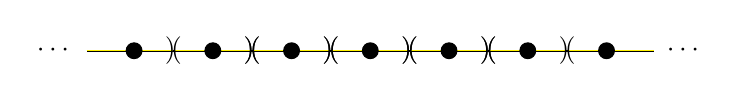
\begin{tikzpicture}
        \draw[step=1, black, thick] (-3.6, 0) -- (3.6, 0);
        \draw[yellow] (-3.6, 0) -- (-2.51, 0);
        \draw[yellow] (2.51, 0) -- (3.6, 0);
        \foreach \x in {-2, -1, 0, 1, 2} {
            \draw[yellow] (\x - 0.49, 0) -- (\x + 0.49, 0);
            \node at (\x - 0.5, 0) {$)\!($};
            \node at (\x + 0.5, 0) {$)\!($};
            \draw[fill=black] (\x, 0) circle (0.1);
        }
        \foreach \x in {-4, 4} {
            \node at (\x,0) {$\cdots$};
        }
        \draw[fill=black] (-3, 0) circle (0.1);
        \draw[fill=black] (3, 0) circle (0.1);
    \end{tikzpicture}
    \caption{The $\Z$ lattice packing in dimension $1$.}
    \label{Ch1:Fig:Z_Lattice_Packing_1D}
\end{figure}

In dimension $2$, \Cref{Ch1:Prob:SpherePacking_n}, also known as the circle packing problem, turns out to be more interesting. A reasonable strategy for finding the densest packing is to `stack' the $\Z$ lattice packing from dimension $1$ onto itself in some manner, turning these intervals into circles of the same radius. The question remains how to do this optimally.

One natural way of doing this is to stack the circles on top of themselves, turning $\Z$ into the lattice $\Z^2$, where circles are centred at points with integer coordinates: see \Cref{Ch1:Subfig:Z2_lattice_packing_2D}. Unfortunately, this packing turns out to be sub-optimal. A better candidate is the $A_2$ lattice packing: see \Cref{Ch1:Subfig:A2_lattice_packing_2D}. This packing is sometimes referred to as the \textit{honeycomb packing} due to the fact that every circle has six neighbours, whose centres form the vertices of a regular hexagon.

It is well-known that the honeycomb packing is optimal in $\R^2$. The original proof of this fact is attributed to Thue \cite{Thue}, but there are many proofs in the literature. One is outlined by Hales in \cite[p. 442]{CannonHoney}. An intuitive way of convincing oneself of Thue's theorem is that it is not possible for a circle in a given row to be in contact with more than $2$ circles in the rows above and below, meaning the $A_2$ packing cannot be improved. See \Cref{Ch1:Subfig:Kepler_Original_1}.

\begin{figure}[htb]
    \centering
    \begin{subfigure}{0.48\linewidth}
        \centering
        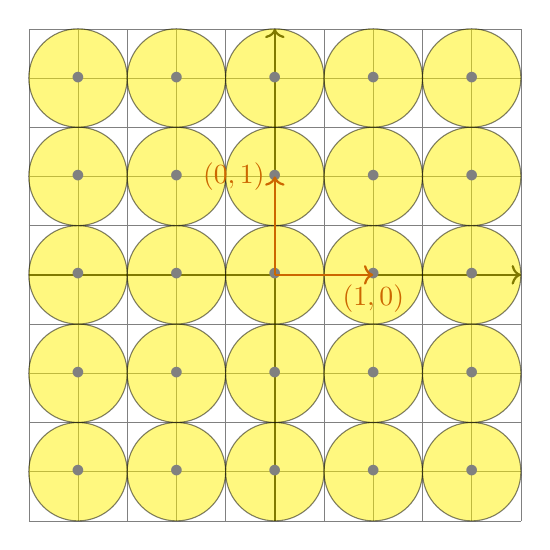
\begin{tikzpicture}[scale=1.25]
            \drawplane
            \foreach \x in {-2, -1, 0, 1, 2} {
                \foreach \y in {-2, -1, 0, 1, 2} {
                    \latticecircle{\x}{\y}
                }
            }
            \draw[->, color=brown, thick] (0,0) -- (1,0) node[anchor=north] {$\parenth{1, 0}$};
            \draw[->, color=brown, thick] (0,0) -- (0,1) node[anchor=east] {$\parenth{0, 1}$};
        \end{tikzpicture}
        \subcaption{The $\Z^2$ lattice packing.}
        \label{Ch1:Subfig:Z2_lattice_packing_2D}
    \end{subfigure}
    \begin{subfigure}{0.48\linewidth}
        \centering
        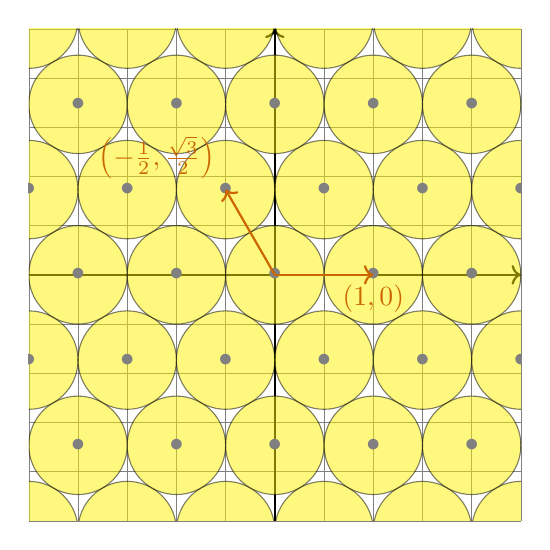
\begin{tikzpicture}[scale=1.25]
            \drawplane
            \clip (-2.5, -2.5) rectangle ++(5, 5);
            \foreach \x in {-4, -3, -2, -1, 0, 1, 2, 3, 4} {
                \foreach \y in {-3, -2, -1, 0, 1, 2, 3} {
                    \latticecircle{\x - \y * 0.5}{\y * 0.8660254038}
                }
            }
            \draw[->, color=brown, thick] (0,0) -- (1,0) node[anchor=north] {$\parenth{1, 0}$};
            \draw[->, color=brown, thick] (0,0) -- (-0.5,0.8660254038) node[anchor=south east] {$\parenth{-\frac{1}{2}, \frac{\sqrt{3}}{2}}$};
        \end{tikzpicture}
        \subcaption{The $A_2$ lattice packing.}
        \label{Ch1:Subfig:A2_lattice_packing_2D}
    \end{subfigure}
    \caption{Circle packings covering the square $\setst{\parenth{x, y} \subset \R^2}{-2.5 \leq x, y \leq 2.5}$.}
    \label{Ch1:Fig:Circle_Packings_2D}
\end{figure}

In dimension $3$, too, it is tempting to replicate this strategy: we can stack the $A_2$ packing on top of itself, in layers instead of rows, attempting to maximise the number of neighbours of a sphere. From trial and error, we see that a sphere cannot be in contact with more than three neighbours from the layer below. This suggests that the optimal sphere packing in dimension $3$ is given by stacking honeycomb arrangements on top of each other with spheres in each layer being nestled in the gaps between three spheres in the layer below.

\begin{wrapfigure}[28]{r}{0.27\linewidth}
    \centering
    \begin{subfigure}{\linewidth}
        \centering
        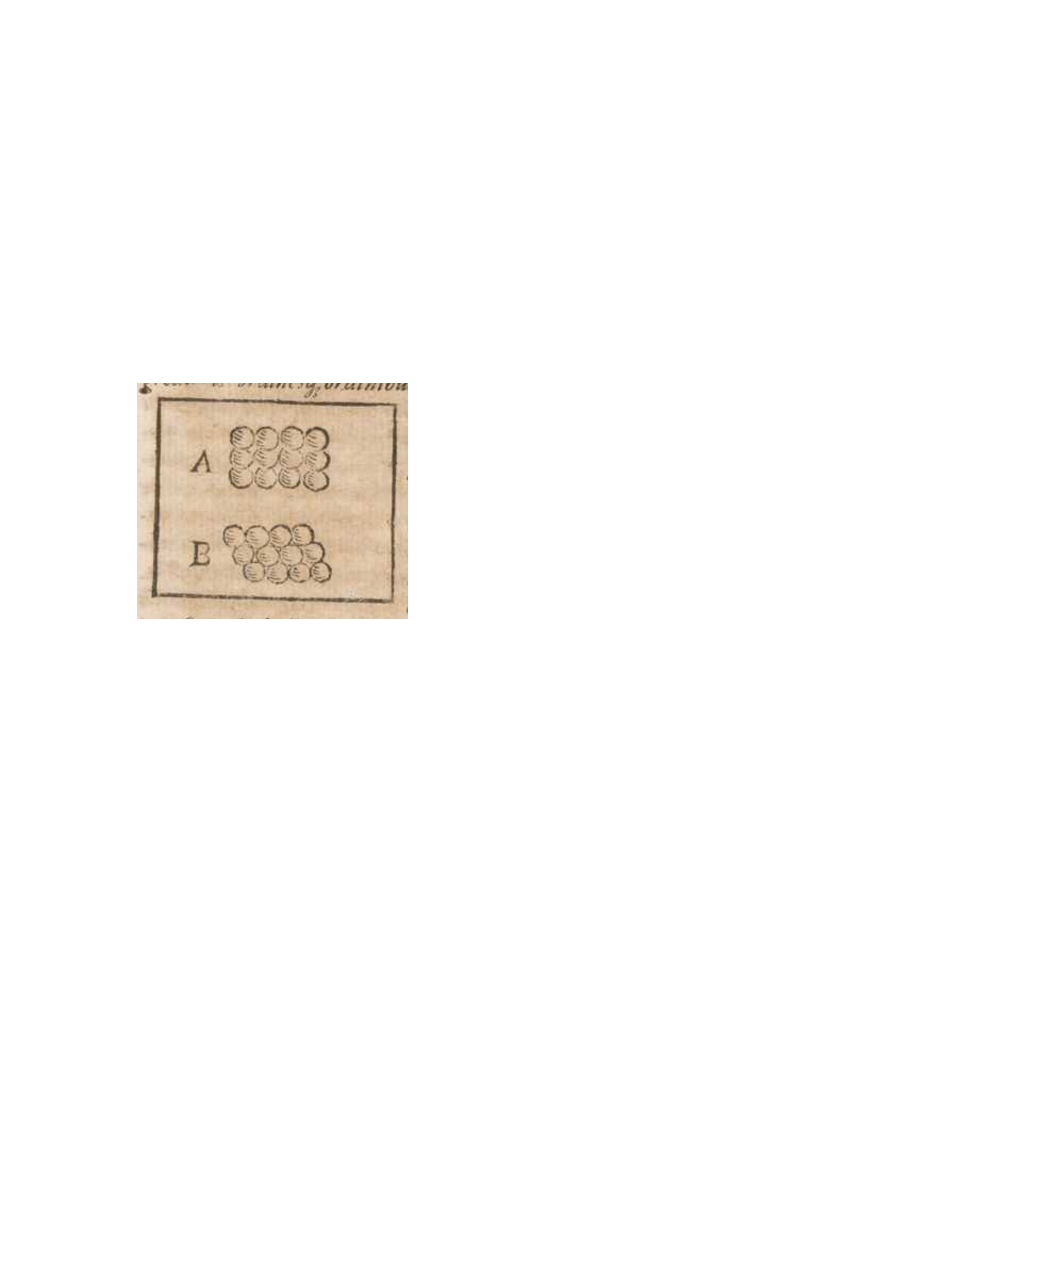
\includegraphics[width=\linewidth]{Chapters/1_Intro/Images/Kepler_1.pdf}
        \caption{}
        \label{Ch1:Subfig:Kepler_Original_1}
    \end{subfigure}
    \begin{subfigure}{\linewidth}
        \centering
        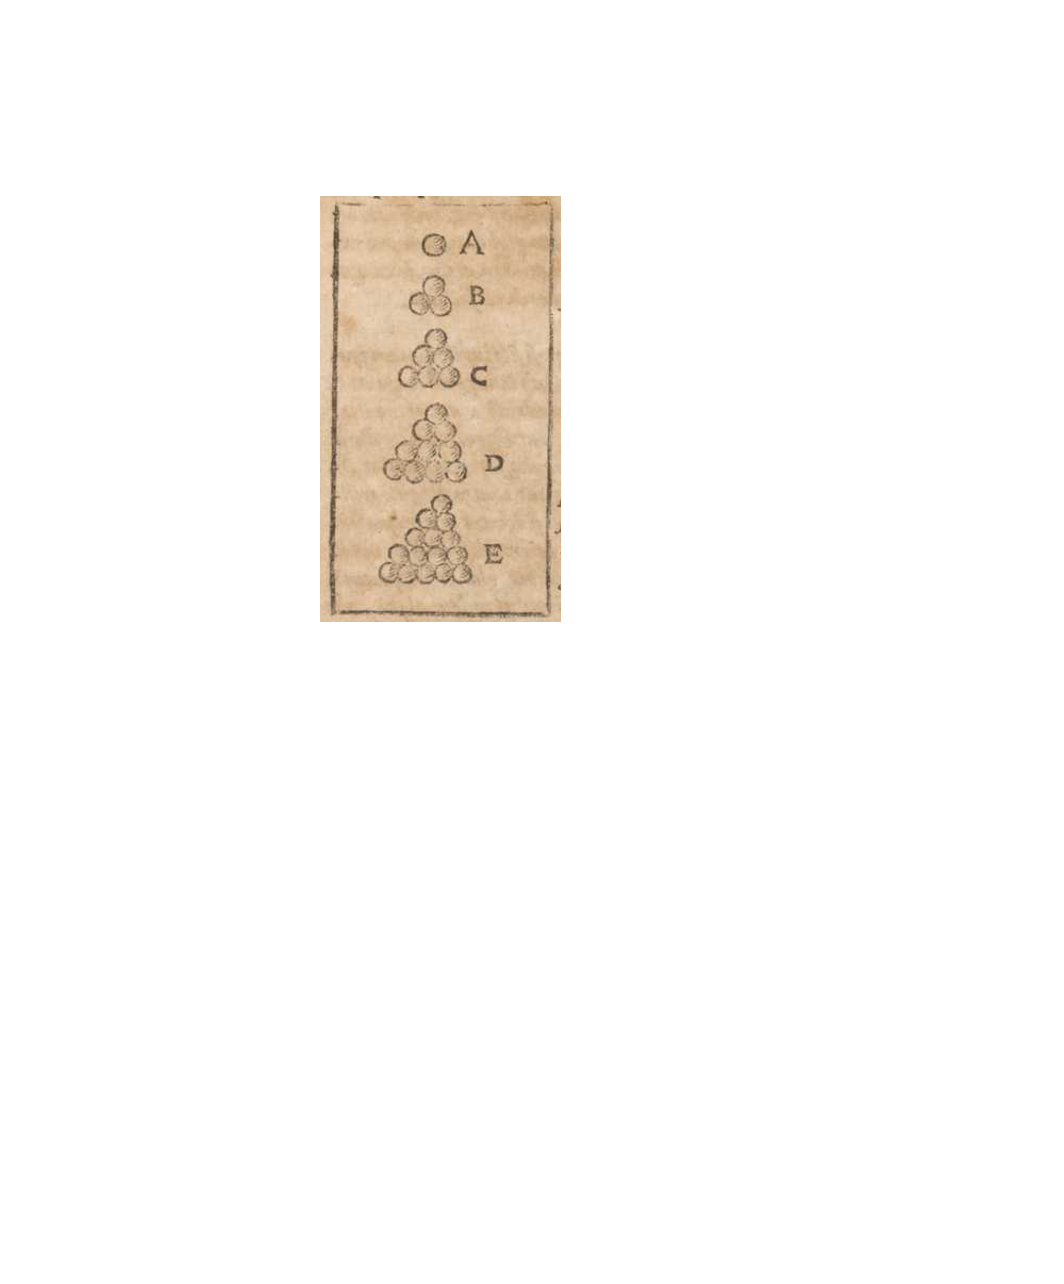
\includegraphics[width=\linewidth]{Chapters/1_Intro/Images/Kepler_2.pdf}
        \caption{}
        \label{Ch1:Subfig:Kepler_Original_2}
    \end{subfigure}
    \caption{Diagrams from an essay written by Johannes Kepler in Latin in 1611 \cite{KeplerSnowflake}.}
\end{wrapfigure}

As it turns out, unlike dimension $2$, this characterisation not describe a unique packing: spheres are simply too large! See \Cref{Ch1:Fig:2_Optimal_3D_Packings}. One can construct infinitely many locally similar, globally different sphere packings in $\R^3$, all of which are as dense as possible, by varying how successive layers are placed.

\begin{figure}[bt]
    \centering
    \begin{subfigure}{0.48\linewidth}
        \centering
        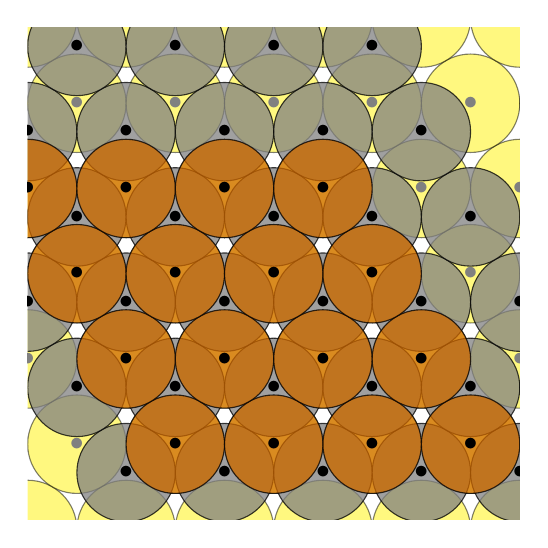
\begin{tikzpicture}[scale=1.25]
            \clip (-2.5, -2.5) rectangle ++(5, 5);
            \foreach \x in {-4, -3, -2, -1, 0, 1, 2, 3, 4} {
                \foreach \y in {-3, -2, -1, 0, 1, 2, 3} {
                    \latticecircle{\x - \y * 0.5}{\y * 0.8660254038}
                }
            }
            \foreach \x in {-3, -2, -1, 0, 1, 2} {
                \foreach \y in {-3, -2, -1, 0, 1, 2} {
                    \latticecirclegrey{\x - \y * 0.5}{\y * 0.8660254038 + 0.5773502692}
                }
            }
            \foreach \x in {-2, -1, 0, 1} {
                \foreach \y in {-2, -1, 0, 1} {
                    \latticecirclebrown{\x - \y * 0.5}{\y * 0.8660254038}
                }
            }
        \end{tikzpicture}
        \subcaption{}
        \label{Ch1:Subfig:3D_Triangular_Stacking}
    \end{subfigure}
    \begin{subfigure}{0.48\linewidth}
        \centering
        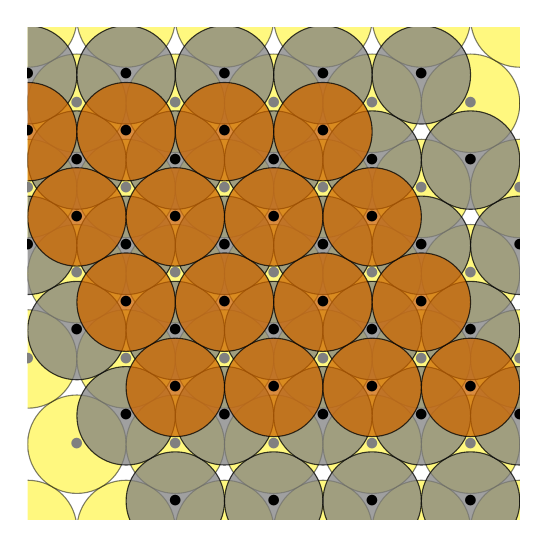
\begin{tikzpicture}[scale=1.25]
            \clip (-2.5, -2.5) rectangle ++(5, 5);
            \foreach \x in {-4, -3, -2, -1, 0, 1, 2, 3, 4} {
                \foreach \y in {-3, -2, -1, 0, 1, 2, 3} {
                    \latticecircle{\x - \y * 0.5}{\y * 0.8660254038}
                }
            }
            \foreach \x in {-2, -1, 0, 1, 2, 3} {
                \foreach \y in {-2, -1, 0, 1, 2, 3} {
                    \latticecirclegrey{\x - \y * 0.5}{\y * 0.8660254038 - 0.5773502692}
                }
            }
            \foreach \x in {-2, -1, 0, 1} {
                \foreach \y in {-2, -1, 0, 1} {
                    \latticecirclebrown{\x - \y * 0.5}{\y * 0.8660254038 + 0.5773502692}
                }
            }
        \end{tikzpicture}
        \subcaption{}
        \label{Ch1:Subfig:3D_Hexagonal_Stacking}
    \end{subfigure}
    \caption{Two different ways of stacking the honeycomb packing on itself.}
    \label{Ch1:Fig:2_Optimal_3D_Packings}
\end{figure}

This observation is not novel. In a 1611 essay whose title has been translated from Latin as \textit{The Six-Cornered Snowflake} \cite{KeplerSnowflake}, Johannes Kepler asserted that spheres cannot be more tightly packed together than they are in a tetrahedral arrangement: see \Cref{Ch1:Subfig:Kepler_Original_2}. This result became known as the Kepler Conjecture, and it went unproven for over three centuries, until 2005 that a paper proving it, written by Thomas Hales, was published \cite{HalesKeplerInformal}.

The complexity of the sphere packing problem in dimension $3$ is illustrated not only by the time elapsed between Kepler's original assertion and a proof being published but also by the length of Hales's paper. Indeed, in an expository account of his proof published in 2000, five years before the publication of the full paper in the Annals, Hales recounted how a jury of twelve referees, despite having been in deliberation for over a year, had yet to make a ``thorough, independent check of the computer code'' he had written to perform the elaborate calculations on which ``every aspect of [his proof] is based'' \cite{CannonHoney}. In January 2003, at the Joint Math Meetings in Baltimore, USA, Hales announced that he intended to formally verify his proof \cite{HalesKeplerFormal}, in what he termed the Flyspeck project. The paper authored by Hales and his collaborators on their successful formalisation of his argument was only published in 2017. Therefore, not only did the Kepler Conjecture take close to 400 years to solve, but it took nearly two decades to eliminate any doubt as to the correctness of the solution. This project aims to formalise a result of a similar flavour in a significantly shorter timeframe.
\section{The Work of Maryna Viazovska}
\section{The Formalisation Movement}
\section{Progress in Formalising Viazovska's Solution in Dimension $8$}

% Do I want to turn this into a separate chapter and toss in section 1.5?
\section{The Scope of this Project}
\chapter{The Ingredients of Viazovska's Solution}
\thispagestyle{empty}
% It might be worth chucking a large part of this chapter into an appendix. Specifically, §2.1.1 (Sphere Packing Fundamentals) and §2.3 (Modular Forms). Need to think about this... this would also depend on how we phrase §1.3 (scope of project) because we need to make it EXTREMELY CLEAR that the purpose of this project was NOT to delve deep into a cool application of the theory of modular forms but rather to learn how to formalise modern, computationally involved mathematics.

The purpose of this chapter is to offer background information that will be essential to understanding the rest of this exposition. We will begin by providing precise mathematical definitions for sphere packings, densities, and the sphere packing constant. We will then discuss the variation of the linear programming bound proven by Cohn and Elkies \cite[Theorem 3.1]{CohnElkies} used by Viazovska \cite[Theorem 2]{Viazovska8}. Finally, we will include a small discussion on the theory of modular forms and establish its relevance to the subsequent chapters of this thesis, which will focus on the construction of the Magic Function.

We will be minimalistic in our discussions, and focus on motivating new concepts and their relevance to the sphere packing problem in dimension $8$. This section is not intended to offer an exhaustive treatment of the mathematics we will encounter, which is as vast as it is rich.

\section{Preliminaries}

Before we begin defining things formally, we must include a small disclaimer about the terminology we have been using---and will continue to use---in this project. While \Cref{Ch1:Prob:SpherePacking_n} is usually referred to as the \textit{sphere} packing problem, a sphere is not usually thought to have an interior. Typically, in any metric space $X$ with metric $d$, the \textit{sphere} of radius $r \geq 0$ centred at $x \in X$ is defined to be $\setst{y \in X}{d(x, y) = r}$. In other words, the sphere consists only of a surface. In contrast, the sphere packing problem involves packing \textit{solid balls}. One can see why, in \cite{CannonHoney}, Hales opines that a more proper term for the problem would be the \textit{ball packing problem}. Nevertheless, in this project, we will continue to use the standard terminology, but we include this disclaimer so the reader bears in mind two things: first, that we will often mean `ball' when we use the word `sphere', and second, that we work with balls instead of spheres in Lean. We will also mention that it is convenient to require that the balls in question be open, so that the condition that spheres cannot overlap but merely touch tangentially can be shortened to that of disjointedness. We introduce notation.

\begin{boxnotation}
    For some $d \in \N$, $x \in \R^d$ and $r > 0$, we denote
    \begin{align*}
        B_d(x, r) := \setst{y \in \R^d}{\norm{x - y} < r}
    \end{align*}
\end{boxnotation}

We organise this section into three subsections. The first defines fundamental notions about sphere packings. The second introduces the properties of two important, and closely related, classes of sphere packings, namely, lattice packings and periodic packings. The third subsection studies the most important sphere packing for our project: the $E_8$ lattice packing.

\subsection{Sphere Packing Fundamentals}

We begin by defining a sphere packing. As we have stated, we want sphere packings to consist of disjoint spheres of the same radius. Given that lying on the interior of a certain sphere corresponds to being within some distance from its centre, we can capture this notion of disjointedness by imposing a separation condition on the set of centres of the sphere packing.

\begin{boxdefinition}[Sphere Packing]
    Fix $d \in \N$ and $X \subset \R^d$. Assume that there exists a real number $r > 0$, known as the \textbf{separation radius}, such that
    \begin{align*}
        \norm{x - y} \geq r
    \end{align*}
    for all distinct $x, y \in X$. We define the \textbf{sphere packing with centres at $X$} to be
    \begin{align*}
        \Pa(X) := \bigcup_{x \in X} B_d(x, r)
    \end{align*}
\end{boxdefinition}

Note that the assumption that a separation radius exists is very important.

\begin{boxnexample}
    Let $d = 1$ and $X = \R$. Consider the set
    \begin{align*}
        \bigcup_{x \in \R} B_1(x, r) = \bigcup_{x \in \R} \parenth{x-r, x+r}
    \end{align*}
    For any $r > 0$, the above union is all of $\R$. However, it does not make sense to construct a sphere packing whose set of centres is the entirety of $\R$, as this would involve spheres overlapping. It is precisely to avoid such constructions that we impose the condition that $r$ be a separation radius on the set of centres.
\end{boxnexample}

Since all the information about a sphere packing is encoded in its set of centres and the corresponding separation radius (which must exist in order for the set of centres to be a valid set of centres for a sphere packing), we decided that a sphere packing would be formalised purely as a set of centres with a valid separation, and that a separate definition would be made to obtain the open balls that constitute the packing. We packaged the data of
\begin{itemize}
    \item the set of centres
    \item the separation radius
    \item the (automatically checked) condition that the separation radius is positive
    \item the condition that the set of centres is, indeed, separated by this radius
\end{itemize}
into a \verb|structure| called \verb|SpherePacking|: see \cite[\texttt{SpherePacking.Basic.SpherePacking}]{documentation}.\todo{Is this an acceptable way of citing the documentation? Should the repo be made public?}

We now define finite density, an indicator of how much of a bounded region of space a sphere packing covers.

\begin{boxdefinition}[Finite Density]\label{Ch2:Def:FiniteDensity}
    Let $\Pa$ be a sphere packing. For all $R > 0$, define the \textbf{finite density} to be
    \begin{align*}
        \Delta_\Pa(R) := \frac{\Volof{\Pa \cap B_d(0, R)}}{\Volof{B_d(0, R)}}
    \end{align*}
    where $\Vol$ is the Lebesgue measure on $\R^d$.
\end{boxdefinition}

Finite density is a somewhat local notion, in that it expresses sphere how closely packed spheres are in a bounded region. The sphere packing problem, on the other hand, examines the notion of closeness on a more global level. While taking the limit of finite densities as the radius of the bounding region approaches infinity might seem like a natural way to define density, it is not obvious that this limit always exists. Therefore, we define density to be the limit superior instead.

\begin{boxdefinition}[Density]\label{Ch2:Def:Density}
    Let $\Pa$ be a sphere packing. Define the \textbf{density} of $\Pa$ to be
    \begin{align*}
        \Delta(\Pa) := \limsup_{R \to \infty} \Delta_\Pa(R)
    \end{align*}
    where $\Delta_\Pa(R)$ is the finite density of $\Pa$, as defined in \Cref{Ch2:Def:FiniteDensity}.
\end{boxdefinition}

As one might expect, finite density and density are invariant under scaling.

\begin{boxproposition}\label{Ch2:Prop:Scaling_Sphere_Packings}
    Let $\Pa$ be a sphere packing. Fix $\lambda > 0$. Denoting by $\lambda \Pa$ the sphere packing obtained by scaling the spheres and the set of centres in $\Pa$ by a factor of $\lambda$, we have
    \begin{align*}
        \Delta_{\Pa}\of{R} = \Delta_{\lambda \Pa}\of{\lambda R}
    \end{align*}
    for all $R > 0$. Similarly, we have
    \begin{align*}
        \Delta\of{\Pa} = \Delta\of{\lambda \Pa}
    \end{align*}
\end{boxproposition}

The sphere packing problem asks for the sphere packing that achieves the highest possible density. We can be formal about the notion of the highest possible density.

\begin{boxdefinition}[Sphere Packing Constant]
    The \textbf{sphere packing constant} in $\R^d$, for any $d > 0$, is defined to be
    \begin{align*}
        \Delta_d := \sup\!\parenth{{\setst{\Delta_{\Pa}}{\Pa \text{ is a sphere packing in } \R^d}}}
    \end{align*}
\end{boxdefinition}

\Cref{Ch2:Prop:Scaling_Sphere_Packings} tells us that it suffices to take the supremum over sphere packings of separation $1$, because a sphere packing $\Pa$ can be scaled down by its separation radius to obtain a sphere packing of separation $1$.

\begin{boxproposition}\label{Ch2:Prop:Scaling_Sphere_Packing_Constant}
    For all $d$, we have
    \begin{align*}
        \Delta_d = \sup\!\parenth{{\setst{\Delta_{\Pa}}{\Pa \text{ is a sphere packing in } \R^d \text{ with separation } 1}}}
    \end{align*}
\end{boxproposition}

As intuitive as this result might seem, we do mention it here because it is something we have to deal with explicitly when formalising the theory of sphere packings in Lean. The first instance when we really see it in action is the proof of \Cref{SP:Thm:CohnElkies}.

The objective of the sphere packing problem in any dimension $d$ is to optimise the sphere packing constant $\Delta_d$. As we have seen, this is a highly non-trivial thing to do. We can, however, offer a trivial upper-bound on sphere packing density.

\begin{boxlemma}
    For any sphere packing $\Pa$ and $R > 0$, we have that $\Delta_{\Pa}(R) \leq 1$.
\end{boxlemma}
\begin{proof}
    This is an immediate consequence of the fact that $\Pa \cap B_d(0, R) \subseteq B_d(0, R)$.
\end{proof}
This immediately gives us the following basic facts.
\begin{boxcorollary}
    For any sphere packing $\Pa$, we have that $\Delta_{\Pa} \leq 1$.
\end{boxcorollary}
\begin{boxcorollary}
    For any $d \in \N$, $\Delta_d \leq 1$.
\end{boxcorollary}

This is not a very good upper-bound. However, it tells us that the sphere packing constant in any number of dimensions is a finite real number in the interval $(0, 1]$. There is still some work to be done before we can give better bounds on the sphere packing constant. Furthermore, it is unclear whether the sphere packing constant actually is, for a general $d$, the density of a sphere packing in $\R^d$. Nevertheless, this is a good starting point.

A great deal of basic sphere packing API in Lean was developed in July 2024 for the project to formalise Viazovska's solution in dimensino $8$. The majority of the code was written by Gareth Ma, who also made significant improvements to the design choices I had made when setting up the project. The definitions and results in this section have all been formalised, and information about the code that has been written can be found in the project documentation \cite[\texttt{SpherePacking.Basic.SpherePacking}]{documentation}.

In the next subsection, we discuss a special class of sphere packings that have periodicity properties with respect to lattices.

\subsection{Lattice and Periodic Sphere Packings}

We begin by defining lattices and briefly commenting on existing \verb|Mathlib| API on lattices. There are primarily two ways in which lattices are defined in mathematical literature. A lattice in some Euclidean space $\R^n$ is either described as the $\Z$-span of some $\R$-basis of $\R^n$ or as a discrete, co-compact subgroup. One can borrow characteristics from both definitions to construct other equivalent definitions.

The characteristics described in both definitions do exist \verb|Mathlib|. However, given that one of the objectives of creating a unified mathematics library is centralisation, a combination of these definitions is used as the \textit{definition} of a \verb|class| that we call \verb|IsZLattice| and information about its many properties, as well as the $\Z$-span construction, are encoded in theorems. In particular, we have a theorem that tell us that every lattice is a free $\Z$-submodule, meaning it has a $\Z$-basis, and that this $\Z$-basis is actually an $\R$-basis of the ambient space. Furthermore, we have a result that every object constructed in that manner is a lattice. Results about types bearing the \verb|IsZLattice| class (ie, lattices as they are defined in \verb|Mathlib|) live in the \verb|ZLattice| namespace, whereas results bout $\Z$-spans of $\R$-bases live in the \verb|ZSpan| namespace. \todo{Create citation for Mathlib.}

We begin by stating the \verb|Mathlib| definition of a lattice.

\begin{boxdefinition}[Lattice]
    A \textbf{lattice} in a Euclidean space $\R^n$ is a discrete $\Z$-submodule of $\R^n$ such that its $\R$-span contains every element in $\R^n$.
\end{boxdefinition}

The \verb|Mathlib| definition is more general, and works for any normed vector space over a normed field. Here, the word `discrete' means that the lattice is discrete in a topological sense, meaning that the subspace topology on the lattice is precisely the discrete topology.

\begin{boxdefinition}[Periodic Sphere Packing]
    Let $\Lambda \subset \R^d$ be a lattice. We say a sphere packing $\Pa(X)$ with spheres centred at points in $X \subset \R^d$ is \textbf{periodic with respect to $\Lambda$}, or \textbf{$\Lambda$-periodic},
    \begin{align*}
        \lambda + X = X
    \end{align*}
    ie, for all $\lambda \in \Lambda$ and $x \in X$, we have that $\lambda + x \in X$.
\end{boxdefinition}

We define Periodic Sphere Packings in Lean as extending the definition of Sphere Packings by creating a \verb|structure| called \verb|PeriodicSpherePacking| that packages the additional data of
\begin{itemize}
    \item the lattice, viewed as a $\Z$-submodule of the ambient space $\R^d$
    \item the condition that the set of centres is periodic with respect to this $\Z$-submodule
    \item the (automatically checked) condition\footnotemark{} that the $\Z$-submodule is discrete
    \item the (automatically checked) condition\footnotemark[\value{footnote}] that the discrete $\Z$-submodule is a lattice
\end{itemize}
\footnotetext{more precisely, the automatically inferred instance}
The definition is in \cite[\texttt{SpherePacking.Basic.SpherePacking}]{documentation}.

Lattice packings are a special class of periodic packings.

\begin{boxdefinition}[Lattice Packing]
    Let $\Lambda \subset \R^d$ be a lattice. The \textbf{$\Lambda$ lattice packing} is the sphere packing with centres at points in $\Lambda$. Such a sphere packing admits a separation radius because $\Lambda$ is discrete and is $\Lambda$-periodic because $\Lambda$ is closed under addition.
\end{boxdefinition}

In \Cref{Ch2:Subsec:E8}, we will briefly examine a specific lattice packing, the $E_8$ lattice packing.

The periodicity property of a periodic sphere packing can be exploited to derive a more convenient formula for its density.

\begin{boxproposition}\label{Ch2:Prop:Periodic_Density}
    Let $\Pa(X)$ be a sphere packing with centres at $X \subset \R^d$ and separation $r$ that is periodic with respect to some lattice $\Lambda \subset \R^d$. We have that
    \begin{align}
        \Delta_{\Pa(X)} = \abs{\quotient{X}{\Lambda}} \frac{\Volof{B_d\of{0, \frac{r}{2}}}}{\Volof{\quotient{\R^d}{\Lambda}}}
        \label{Ch2:Eq:Periodic_Density}
    \end{align}
\end{boxproposition}

The proof is beyond the scope of this M4R project, but was formalised in Summer 2024: see \verb|PeriodicSpherePacking.density_eq'| in \cite[\texttt{SpherePacking.Basic.PeriodicPacking}]{documentation}.

Just as we defined the sphere packing constant for any dimension $d \in \N$, we can define a \textit{periodic} sphere packing constant in any dimension.

\begin{boxdefinition}[Periodic Sphere Packing Constant]
    For all $d \in \N$, define the \textbf{periodic sphere packing constant in dimension $d$} to be
    \begin{align*}
        \Delta_{d}^{\periodic} = \sup\of{{\setst{\Delta_{\Pa}}{\Pa \text{ is a periodic sphere packing in } \R^d}}}
    \end{align*}
\end{boxdefinition}

The power of periodic sphere packings is illustrated by a rather surprising fact.

\begin{boxproposition}\label{Ch2:Prop:Periodic_Const_eq_Const}
    For all $d \in \N$,
    \begin{align*}
        \Delta_{d} = \Delta_{d}^{\periodic}
    \end{align*}
\end{boxproposition}

We do not prove this result here, as it is beyond the scope of this M4R. A proof can be found in \cite[Appendix A]{CohnElkies}. We do, however, mention that \Cref{Ch2:Prop:Periodic_Const_eq_Const} can be combined with \Cref{Ch2:Prop:Scaling_Sphere_Packing_Constant} to give the following.

\begin{boxproposition}\label{Ch2:Prop:Scaling_Periodic_Constant}
    For all $d \in \N$,
    \begin{align*}
        \Delta_{d} = \sup\of{{\setst{\Delta_{\Pa}}{\Pa \text{ is a periodic sphere packing in } \R^d \text{ with separation } 1}}}
    \end{align*}
\end{boxproposition}

\Cref{Ch2:Prop:Periodic_Const_eq_Const} tells us that finding a sphere packing that satisfies the \textit{periodic} sphere packing constant gives us the optimal sphere packing in dimension $d$. \Cref{Ch2:Prop:Scaling_Periodic_Constant} allows us to focus our search even more. We will exploit these two facts in \Cref{Ch2:Sec:CohnElkies}, where we will construct an upper bound for all sphere packing densities in dimension $d$ by constructing an upper-bound for the periodic sphere packing constant in dimension $d$. When constructing this upper-bound, we will exploit the fact that periodic sphere packings admit a `nice' density formula (cf. \Cref{Ch2:Prop:Periodic_Density}). The results we have seen about periodic sphere packings will thus greatly simplify our task of finding the optimal sphere packing in dimension $8$.

We are now ready to discuss a special sphere packing in $\R^8$: the $E_8$ sphere packing.

\subsection{The $E_8$ Lattice Packing}\label{Ch2:Subsec:E8}

\begin{wrapfigure}[18]{r}{0.5\linewidth}
    \vspace{-3em}
    \centering
    \includegraphics[width=0.98\linewidth]{Chapters/2_Dimension_8/Images/Gorbe_E8.png}
    \caption{The Coxeter projection of the $E_8$ root system. \cite{Gorbe_E8}}
    \label{Ch2:Fig:Gorbe_E8}
\end{wrapfigure}

It is quite remarkable that $E_8$ should show up when discussing sphere packings. At its core, $E_8$ is an irreducible root system. It shows up in the classification of important classes of objects like irreducible Coxeter groups, crystallographic Coxeter groups, and semi-simple Lie algebras over $\C$. $E_8$ is not a classical root system but an \textit{exceptional} root system, meaning that the geometric properties of its roots cannot be found in irreducible root systems in all dimensions.

The $E_8$ root system consists of $240$ vectors in $\R^8$ that are permuted by a certain finite subgroup of the $8$-dimensional orthogonal group. This group is sometimes referred to as the $E_8$ Coxeter group or as the Weyl group of the $E_8$ lattice. These roots can be divided into $8$ orbits, each of which corresponds to one of the `layers' of concentric circles in \Cref{Ch2:Fig:Gorbe_E8}. The dots in the figure correspond to projections of the roots onto a plane on which a specific type of element of the Coxeter group, known as a Coxeter element, acts as a rotation. This visualisation offers a convenient---and aesthetically pleasing---means of visualising this collection of $8$-dimensional vectors and appreciating some of its symmetry.

% From a motivational standpoint, this is quite important. So mention facts like distances between lattice points and things like that. Important for construction of magic function.



\section{The Cohn-Elkies Linear Programming Bounds}
\section{A Word on Modular Forms}
\label{Ch2:Sec:ModForms}
% SHOULD I MAYBE TURN THIS INTO AN APPENDIX? IT'S LOOKING PRETTY LONG...

\begin{comment}
Things to discuss:
1. What is a modular form
2. What is a quasimodular form
3. Examples: Eisenstein Series, Jacobi Theta functions, Discriminant form
We can reference things like the q-expansions of the Eisenstein series, the transformation rules for the Jacobi theta functions, and the product formula for the discriminant form.
\end{comment}

In this section, we give a brief introduction to the theory of modular forms. Birkbeck, Loeffler and others have formalised several results in the theory of modular forms, and a significant portion of their work has been merged into \mathlib. Definitions and results from this section that pertain to Viazovska's solution to the sphere packing problem in $\R^8$ that do not feature in \mathlib\ are being actively formalised by Birkbeck and Lee, with contributions from Ma.

First, we introduce the following useful notation.

\begin{boxnotation}
    For the remainder of this paper, denote the Complex upper half-plane by $\Halfplane$. That is, define $\Halfplane := \setst{z \in \C}{0 < \Im(z)}$.
\end{boxnotation}

This corresponds to the \mathlib\ notation for the upper half-plane.

A key motivating idea in the study of modular forms is the study of the action of $\SL{2, \Z}$ on $\Halfplane$ by Möbius transformations via
\begin{align*}
    \begin{bmatrix}
        a & b \\ c & d
    \end{bmatrix}
    \cdot z := \frac{az + b}{cz + d}
\end{align*}
That matrix multiplication corresponds to the composition of Möbius transformations is a well-known fact in Complex Analysis. One can hence show that the above is indeed a group action.

Both the identity $I \in \SL{2, \Z}$ and the negative identity $-I \in \SL{2, \Z}$ have the same (trivial) action on $\Halfplane$. Indeed, the $\SL{2, \Z}$ action descends to a faithful action of $\PSL{2, \Z} = \quotient{\SL{2, \Z}}{\set{\pm I}}$ on $\Halfplane$. Since we are more interested in the \textit{actions} of matrices in $\SL{2, \Z}$ and $\PSL{2, \Z}$ than we are in their entries, we often do not distinguish between the two groups.

The \mathlib\ definition of a modular form is more general than the first definitions of modular forms often seen in literature (see \cite[Chapter VII, \S 2, Definition 4]{SerreArith} and \cite[Definition 1.1.2]{DiamondShurman}), and instead matches subsequent definitions that generalise these first definitions. Modular forms are usually described as functions that are holomorphic on the upper half-plane that are invariant under the $\SL{2, \Z}$-action up to an \textit{automorphy factor} of a certain \textit{weight}. This \textit{weight} is defined as the \textit{weight of the modular form}. However, one is often interested in invariance under not all of $\SL{2, \Z}$, but certain \textit{principal congruence subgroups} or subgroups containing such subgroups, known as \textit{congruence subgroups}. Each principal congruence subgroup has a \textit{level}, which is defined to be the \textit{level} of a modular form whose congruence subgroup is principal. Modular forms, as they are defined in \mathlib\ and in the blueprint \cite{blueprint}, are therefore indexed by two properties: a \textit{congruence subgroup of $\SL{2, \Z}$}, which indicates the scope of invariance under the $\SL{2, \Z}$-action, and a \textit{weight}, which gives the extent of invariance under the action of elements of the subgroup in question.

To give a complete definition of the weight of a modular form, we need to define automorphy factors and the slash action notation.

\begin{boxdefinition}[Automorphy Factors and Slash Actions]\label{Ch2:Def:Aut_Factor_Slash_Action}
    Fix $k \in \Z$, $z \in \Halfplane$ and $\gamma = \begin{bmatrix} a & b \\ c & d \end{bmatrix} \in \SL{2, \Z}$. Define the \textbf{automorphy factor of weight $k$} to be
    \begin{align}
        j_k\of{z, \gamma} &:= \parenth{cz + d}^{-k}
        \label{Ch2:Eq:AutomorphyFactor_def}
    \end{align}
    For any function $f : \Halfplane \to \C$, with $k$ and $\gamma$ as above, the \textbf{slash operator} maps $f$ to a new function $f \mid_k \gamma : \Halfplane \to \C$ given by
    \begin{align}
        \fmof{k}{\gamma}{z} &:= j_k\of{z, \gamma} \fof{\gamma \cdot z} = \parenth{cz + d}^{-k} \fof{\frac{az + b}{cz + d}}
        \label{Ch2:Eq:SlashAction_def}
    \end{align}
    The action of $\gamma$ mapping $f$ to $\fm_k \gamma$ via the weight $k$ slash operator is sometimes referred to as a \textbf{slash action}.
\end{boxdefinition}

It is clear, from the above definition, that $\fm_0 \gamma = f \circ \gamma$ for al $\gamma \in \SL{2, \Z}$. That is, if $f = \fm_0 \gamma$, then $f = f \circ \gamma$, that is, $f$ is invariant under composition with (the action of) $\gamma$. If $f = \fm_k \gamma$ for some $k \in \Z$ and $\gamma \in \SL{2, \Z}$, we can view the weight $k$ as indicating the `extent of invariance' of $f$ under composition with $\gamma$. Note that slash actions can be composed.

\begin{boxlemma}\label{Ch2:Lemma:Slash_Mul}
    For all $k \in \Z$, $f : \Halfplane \to \C$ and $\gamma_1, \gamma_2 \in \SL{2, \Z}$,
    \begin{align*}
        \parenth{f \mid_k \gamma_1} \mid_k \gamma_2 = f \mid_k \parenth{\gamma_1 \gamma_2}
    \end{align*}
    where $\gamma_1 \gamma_2$ is the product of $\gamma_1$ and $\gamma_2$ as matrices.
\end{boxlemma}
A slightly more general version of this has been \href{https://github.com/leanprover-community/mathlib4/blob/a0370507e2922f0a329a2d8cc17e9f9148cd168d/Mathlib/NumberTheory/ModularForms/SlashActions.lean#L77}{formalised} in \mathlib.

We are now ready to define congruence subgroups, which will tell us under precisely which elements of $\SL{2, \Z}$ a modular form is slash-invariant. We express this notion in the language of modular arithmetic.

\begin{boxdefinition}[Congruence Subgroup]\label{Ch2:Def:Cong_Subgroup}
    Fix $N \in \N$. The \textbf{level $N$ principal congruence subgroup} of $\SL{2, \Z}$, denoted $\Gamma(N)$, is defined to be the kernel of the surjective group homomorphism from $\SL{2, \Z}$ to $\SL{2, \Zmod{N}}$ that comes from reducing modulo $N$. That is,
    \begin{align}
        \Gamma(N) &:= \setst{
        \begin{bmatrix}
            a & b \\ c & d
        \end{bmatrix} \in \SL{2, \Z}}{
        \begin{bmatrix}
            a & b \\ c & d
        \end{bmatrix}
        \equiv
        \begin{bmatrix}
            1 & 0 \\ 0 & 1
        \end{bmatrix}
        \pmod{N}}
        \label{Ch2:Eq:PrincipalCongruenceSubgroup_def}
    \end{align}
    More generally, a subgroup $\Gamma$ of $\SL{2, \Z}$ is called a \textbf{congruence subgroup} if $\Gamma(N) \subset \Gamma$ for some $N \in \N$.
\end{boxdefinition}

We now have enough to define what it means for a holomorphic function to be invariant under the slash action of a congruence subgroup. In the definition of modular forms, however, we include an additional condition that is often referred to as \textit{holomorphicity at $i\infty$}, the purpose of which is to ensure that spaces of modular forms, which turn out to admit $\C$-vector space structures, are, in fact, finite-dimensional \cite{KevinFamilies}.

The theory of modular forms is often thought to lie in the very rich intersection of algebra and analysis. Our definitions so far have been largely algebraic, but our next one is analytic. Consider the mapping $q : \Halfplane \to \C : z \mapsto e^{2\pi i z}$. This maps $\Halfplane$ to the punctured, open unit disc
\begin{align*}
    D := \setst{w \in \C}{0 < \abs{q} < 1}
\end{align*}
Indeed, for all $z \in \Halfplane$, writing $z = x + iy$ for $x, y \in \R$ with $y > 0$, we have
\begin{align*}
    \abs{q(z)} = \abs{e^{2 \pi i \parenth{x + iy}}} = \abs{e^{2\pi i x}} \cdot \abs{e^{-2\pi y}} < 1
\end{align*}
with $0 \notin q\of{\Halfplane}$ but $q(z) \to 0$ as $\Im(z) = y \to \infty$. Now, we know that the holomorphic functions from $D \to \C$ are precisely those that have Laurent expansions of the form
\begin{align*}
    \sum_{n=0}^{\infty} c_n w^n
\end{align*}
for all $w \in D$. If we write $w = q(z)$ for $z \in \Halfplane$, the above series turns out to be a \textit{Fourier expansion}. We can hence make the following definition for holomorphicity at $i\infty$.

\begin{boxdefinition}[Holomorphicity at $i\infty$]\label{Ch2:Def:Holo_at_ImInfty}
    We say a function $f : \Halfplane \to \C$ is \textbf{holomorphic at $i\infty$} if $f$ admits a Fourier expansion of the form
    \begin{align*}
        f(z) = \sum_{n=0}^{\infty} c_n q(z)^n = \sum_{n=0}^{\infty} c_n e^{2\pi i nz}
    \end{align*}
    That is, $f$ admits a Fourier expansion with no negative powers of $q(z)$.
\end{boxdefinition}

The holomorphicity of $f$ at $i\infty$ essentially means that the Fourier expansion of $f$ is a holomorphic $D \to \C$ function in $q(z)$, with the added constraint that $\abs{f(z)}$ remains bounded as $\Im(z) \to \infty$, that is, the corresponding $D \to \C$ function in $q(z)$ extends to a holomorphic function that is defined and bounded at $0$. There is a rich theory of functions where $c_0 = 0$, but we will not explore that theory here.\footnote{Modular forms with this property are known as \textbf{cusp forms}. One modular form we will need to construct the magic function is the discriminant form, which will turn out to be a cusp form.}

We are now ready to define modular forms. Intuitively, a modular form is a function that satisfies the above definitions in a slash-invariant manner. More precisely, we have the following.

\begin{boxdefinition}[Modular Form]
    Fix $k \in \Z$ and let $\Gamma$ be a congruence subgroup of $\SL{2, \Z}$. We say a function $f : \Halfplane \to \C$ is a \textbf{modular form of weight $k$ with respect to $\Gamma$} if $f$ is \textbf{invariant} under the slash action of $\Gamma$ and \textbf{holomorphic at $i\infty$} under the slash action of $\SL{2, \Z}$. That is,
    \begin{enumerate}
        \item For all $\gamma \in \Gamma$, $\fm_k \gamma = f$ (cf. \Cref{Ch2:Def:Aut_Factor_Slash_Action}).
        \item For all $\gamma \in \SL{2, \Z}$, $\fm_k \gamma$ is holomorphic at $i\infty$ (cf. \Cref{Ch2:Def:Holo_at_ImInfty}).
    \end{enumerate}
    We denote by $M_k(\Gamma)$ the space of modular forms of weight $k$ and congruence subgroup $\Gamma$. If $\Gamma = \Gamma(N)$ for some $N \in \N$, we say an element of $M_k(\Gamma)$ has \textbf{level $N$}.
\end{boxdefinition}

There is an immensely rich theory of modular forms, and for the purposes of practicality, it was decided not to explore this theory in great detail in this project, particularly because the formalisation of the aspects of Viazovska's proof that stem from this theory is being led by Birkbeck, Lee and Ma. We will instead use the remainder of this section to discuss three specific (families of) modular forms and those of their properties that Viazovska uses to construct her magic function.

\subsection{The Eisenstein Series}
\label{Ch2:Subsec:EisensteinSeries}

The Eisenstein Series are an important family of slash-invariant forms that will prove essential to the construction of the magic function. The Eisenstein Series whose \textit{weight} is an even integer that is at least $4$ are modular forms, though we will also need to work with the Eisenstein Series of weight $2$, which, despite not being a modular form, is sufficiently well-behaved for our purposes. We will define it separately from those Eisenstein Series that are modular forms.

Let $k \geq 4$ be an even integer. We denote by $E_k$ the weight $k$ Eisenstein Series. There is more than one way to define $E_k$. In this report, we give the definition that was formalised by Birkbeck for this project. Birkbeck's definition in the project repository is a particular case of the \href{https://github.com/leanprover-community/mathlib4/blob/70816aec3a0f7bb98ac42991652a66b6405e1a00/Mathlib/NumberTheory/ModularForms/EisensteinSeries/Basic.lean#L28-L35}{\mathlib\ definition}, which defines it as a \texttt{ModularForm} structure combining the function \href{https://github.com/leanprover-community/mathlib4/blob/70816aec3a0f7bb98ac42991652a66b6405e1a00/Mathlib/NumberTheory/ModularForms/EisensteinSeries/Defs.lean#L107}{\texttt{eisensteinSeries}} with the proofs of the properties that make it a modular form. The \mathlib\ definition is more general than the one we study here, and involves imposing congruence conditions on the subsets of the lattice $\Z^2$ over which the Eisenstein Series are summed. It is not necessary for this project.

\begin{boxdefinition}[The Eisenstein Series of Even Weight $\geq 4$]\label{Ch2:Def:EisensteinSeries_geq_4}
    For $k \geq 4$ even, define the \textbf{weight $k$ Eisenstein Series} to be the function $E_k : \Halfplane \to \C$ given by
    \begin{align}
        E_k(z) := \frac{1}{2} \sum_{\substack{\parenth{m, n} \in \Z^2 \\ \gcd(m, n) = 1}} \frac{1}{\parenth{mz + n}^k}
        \label{Ch2:Eq:Eisenstein_def_Chris}
    \end{align}
    with the defining summation converging absolutely.
\end{boxdefinition}

Note that the Eisenstein Series can also be defined as
\begin{align}
    E_k(z) = \frac{1}{2\zeta(k)} \sum_{\parenth{m, n} \in \Z^2 \setminus \set{0}} \frac{1}{\parenth{mz + n}^k}
    \label{Ch2:Eq:Eisenstein_def_with_zeta_normalisation}
\end{align}
with $\zeta$ here denoting the Riemann zeta function. It is shown in \cite[Equation (4.1), pp. 109-110]{DiamondShurman} that this definition matches the definition formalised by Birkbeck in the project repository and stated informally in \Cref{Ch2:Def:EisensteinSeries_geq_4}.\todo{Blueprint gives zeta def whereas repo gives coprime def. WHOOPSIE!}

It is shown in \cite[pp. 4-5]{DiamondShurman} that $E_k$ is a weight $k$, level $1$ modular form for even integers $k \geq 4$. That is, $E_k$ is invariant under the weight $k$ slash-action of every element of $\SL{2, \Z}$. As important special cases of this, $E_k$ satisfies two important functional equations.

\begin{boxproposition}\label{Ch2:Prop:Eisenstein_func_eq}
    For all even $k \geq 4$ and $z \in \Halfplane$, the following both hold:
    \begin{align}
        E_k\of{z + 1} &= E_k \label{Ch2:Eq:Ek_func_eq_one_add} \\
        E_k\of{-\frac{1}{z}} &= z^k E_k(z) \label{Ch2:Eq:Ek_func_eq_neg_one_div}
    \end{align}
\end{boxproposition}
\begin{proof}
    Both of these are just slash-invariance properties in disguise. We have\todo{Fix slash formatting}
    \begin{align*}
        E_k(z + 1) = \parenth{E_k \; \middle\vert_k \; {\begin{bmatrix} 1 & 1 \\ 0 & 1 \end{bmatrix}}}\of{z} = \parenth{0z + 1}^{k} E_k(z) = E_k(z)
    \end{align*}
    Similarly, we have
    \begin{align*}
        E_k\of{-\frac{1}{z}} = \parenth{E_k \; \middle\vert_k \; {\begin{bmatrix} 0 & -1 \\ 1 & 0 \end{bmatrix}}}\of{z} = \parenth{1z + 0}^k E_k(z) = z^k E_k(z)
    \end{align*}
    as required.
\end{proof}

The functional equations \eqref{Ch2:Eq:Ek_func_eq_one_add} and \eqref{Ch2:Eq:Ek_func_eq_neg_one_div} yield similar results for an important function that will be used in constructing the magic function. We will explore this idea in \Cref{Ch4:Chapter}.

One of the most important properties of the Eisenstein Series---at least, for our purposes---is that their Fourier coefficients\footnote{The slash-invariant properties of modular forms mean that they have periodicity properties. Computing their Fourier series is hence a natural strategy when attempting to dissect their properties.} grow polynomially. We will be particularly interested in $E_4$ and $E_6$, which are defined as above, and their cousin $E_2$, which we will treat separately. These functions show up in the definition of Viazovska's magic function, and the polynomial growth property allows us to prove that the magic function is Schwartz.

Our strategy to prove that the Fourier coefficients have polynomial growth will be to compute them explicitly. First, we need to define the arithmetic function $\sigma_k(n)$, which is defined in \mathlib\ as \href{https://github.com/leanprover-community/mathlib4/blob/70816aec3a0f7bb98ac42991652a66b6405e1a00/Mathlib/NumberTheory/ArithmeticFunction.lean#L797-L799}{\texttt{ArithmeticFunction.sigma}}.

\begin{boxdefinition}[The $\sigma$-Function]
    The \textbf{$\sigma$-function} $\sigma : \N \times \N \to \N$ is given by
    \begin{align*}
        \sigma_k\of{n} := \sum_{d \mid n} d^k
    \end{align*}
\end{boxdefinition}

In \mathlib, for every natural number \texttt{k}, \texttt{ArithmeticFunction.sigma k} is defined as an \href{https://github.com/leanprover-community/mathlib4/blob/bc10be4a66942c0fc2547b54f7f8715df72ff28c/Mathlib/NumberTheory/ArithmeticFunction.lean#L76-L80}{\texttt{ArithmeticFunction $\N$}} structure, meaning it is an $\N \to \N$ map that maps $0$ to $0$.

The reason we defined the $\sigma$-function is that the Fourier coefficients of the Eisenstein series are given in terms of $\sigma$.

\begin{boxtheorem}\label{Ch2:Thm:Ek_qexpansion}
    For all even $k \geq 4$ and $z \in \Halfplane$, $E_k(z)$ can be expressed as the Fourier series
    \begin{align}
        E_k(z) &= 1 + C_k \sum_{n=1}^{\infty} \sigma_{k-1}\of{n} e^{2\pi i n z}
        \label{Ch2:Eq:Ek_qexpansion}
    \end{align}
    where
    \begin{align}
        C_k = \frac{1}{\zeta(k)} \cdot \frac{\parenth{-2 \pi i}^k}{\parenth{k-1}!}
        \label{Ch2:Eq:Ck_Ek_qexpansion_const}
    \end{align}
    In particular, $C_4 = 240$ and $C_6 = -504$. That is, $E_4$ and $E_6$ have the following Fourier expansions:
    \begin{align}
        E_4(z) &= 1 + 240 \sum_{n=1}^{\infty} \sigma_3(n) e^{2 \pi i n z} \label{Ch2:Eq:E4_qexpansion} \\
        E_6(z) &= 1 - 504 \sum_{n=1}^{\infty} \sigma_5(n) e^{2 \pi i n z} \label{Ch2:Eq:E6_qexpansion}
    \end{align}
\end{boxtheorem}

The statement and proof of the general Fourier expansion of $E_k$ for even $k \geq 4$ have been \href{https://github.com/thefundamentaltheor3m/Sphere-Packing-Lean/blob/076f4b8d6a37fa95de3bc4764a5d7f911fde91e0/SpherePacking/ModularForms/Eisensteinqexpansions.lean#L301}{formalised by Birkbeck} in the Sphere Packing repository.\todo{Here, again, the repo disagrees with the blueprint. FIX!} Substituting $k = 4$ and $k = 6$ in the expression for $C_k$ and evaluating it using software like Wolfram|Alpha gives the desired result.

Now, it is immediate that the Fourier coefficients exhibit polynomial growth: for all $k, n \in \N$, $\sigma_k(n)$ is a sum of at most $n$ numbers that are each at most $n^k$, meaning $\sigma_k(n) \leq n^{k+1}$.

% TODO: RAISE THIS ON ZULIP. Mention that we need to correct the blueprint to reflect the repo version.

For the remainder of this subsection, we will focus on a cousin of the weight $\geq 4$ Eisenstein Series: the weight $2$ Eisenstein Series, denoted $E_2$. The reason why we treat $E_2$ separately is that it is not a modular form. Furthermore, it cannot be defined via the summation used in \Cref{Ch2:Eq:Eisenstein_def_Chris} or \Cref{Ch2:Eq:Eisenstein_def_with_zeta_normalisation}: unfortunately, when $k = 2$, these sums do not converge absolutely. That being said, Birkbeck has \href{https://github.com/thefundamentaltheor3m/Sphere-Packing-Lean/blob/076f4b8d6a37fa95de3bc4764a5d7f911fde91e0/SpherePacking/ModularForms/summable_lems.lean#L1680}{shown formally} that for all $m \in \Z$, $z \in \Halfplane$, and $k \geq 2$, the summation
\begin{align*}
    \sum_{n \in \Z} \frac{1}{\parenth{mz + n}^k}
\end{align*}
converges absolutely. He then shows, through several \sorry-free lemmas, that
\begin{align*}
    \lim_{N \to \infty} \sum_{m = -N}^{N - 1} \sum_{n \in \Z} \frac{1}{\parenth{mz + n}^k}
\end{align*}
exists, allowing us to define $E_2$ in the following manner.

\begin{boxdefinition}[$E_2$]
    For all $z \in \Halfplane$, define
    \begin{align*}
        E_2(z) := \frac{1}{2\zeta(2)} \lim_{N \to \infty} \sum_{m = -N}^{N - 1} \sum_{n \in \Z} \frac{1}{\parenth{mz + n}^k}
    \end{align*}
\end{boxdefinition}

The difference between this definition and \eqref{Ch2:Eq:Eisenstein_def_with_zeta_normalisation} with $k = 2$ is that here, we specify an order of summation for the outer sum, whereas for $k \geq 4$, in both \eqref{Ch2:Eq:Eisenstein_def_with_zeta_normalisation} and \eqref{Ch2:Eq:Eisenstein_def_Chris}, the order is immaterial due to absolute convergence. Interestingly, the Fourier expansion of $E_2$ agrees with \eqref{Ch2:Eq:Ek_qexpansion}.

\begin{boxtheorem}\label{Ch2:Thm:E2_qexpansion}
    For all $z \in \Halfplane$, $E_2(z)$ can be expressed as the Fourier series
    \begin{align}
        E_2(z) = 1 - 24 \sum_{n=1}^{\infty} \sigma_1(n) e^{2 \pi i n z}
        \label{Ch2:Eq:E2_qexpansion}
    \end{align}
\end{boxtheorem}

Birkbeck gives a formal proof of this over the course of several \sorry-free lemmas in \href{https://github.com/thefundamentaltheor3m/Sphere-Packing-Lean/blob/076f4b8d6a37fa95de3bc4764a5d7f911fde91e0/SpherePacking/ModularForms/E2.lean#L736}{\texttt{SpherePacking.ModularForms.E2.lean}}. Interestingly, substituting $k = 2$ in \eqref{Ch2:Eq:Ck_Ek_qexpansion_const} yields precisely $-24$. Moreover, the same argument we used earlier demonstrates that the Fourier coefficients of $E_2$ also grow polynomially. We will mention this result again in \Cref{Ch4:Chapter}, where we will prove that the magic function is Schwartz.

 We end our discussion on the Eisenstein Series by giving an explicit counterexample to weight $2$, level $1$ slash-invariance that shows that $E_2$ is not a weight $2$, level $1$ modular form.

\begin{boxlemma}\label{Ch2:Lemma:E2_slash_action}
    For all $\gamma = \begin{bmatrix} a & b \\ c & d \end{bmatrix} \in \SL{2, \Z}$, we have
    \begin{align*}
        E_2 \mid_2 \gamma = \parenth{cz + d}^{-2} E_2\of{\frac{az + b}{cz + d}} = E_2(z) - \frac{6ic}{\pi\parenth{cz + d}}
    \end{align*}
\end{boxlemma}

The proof uses results about the discriminant form, which we define in the next subsection. We do not prove the above result here, as it is significantly beyond the scope of this project, but we point the reader to the blueprint \cite[Lemma 6.39]{blueprint}.\todo{Update blueprint reference before submitting}

\subsection{The Discriminant Form}

The discriminant form is a weight $12$, level $1$ modular form. As was briefly alluded to earlier, it is a cusp form. It is defined in terms of the Eisenstein series $E_4$ and $E_6$.

\begin{boxdefinition}[The Discriminant Form]\label{Ch2:Def:DiscForm}
    The \textbf{discriminant form} $\Delta$ is defined by
    \begin{align}
        \Delta := \frac{E_4^3 - E_6^2}{1728}
        \label{Ch2:Eq:DiscForm_def}
    \end{align}
\end{boxdefinition}

The discriminant form has important positivity and non-vanishing properties that we will use repeatedly, either directly or indirectly, in the construction of the magic function. The discriminant form will often show up in denominators, making these properties essential to prove properties like holomorphicity. The key to these properties is the so-called product formula.

\begin{boxtheorem}[Product Formula for $\Delta$]\label{Ch2:Thm:Delta_Product_Formula}
    For all $z \in \Halfplane$, $\Delta(z)$ is expressible as the following infinite product:
    \begin{align}
        \Delta(z) = e^{2 \pi i z} \prod_{n=1}^{\infty} \parenth{1 - e^{2 \pi i n z}}^{24}
    \end{align}
\end{boxtheorem}

% ASK CHRIS ABOUT LEAN PROOF OF PRODUCT FORMULA!

A proof can be found in \cite[Chapter VII, §4, Theorem 6, p. 95]{SerreArith}. Birkbeck has \href{https://github.com/thefundamentaltheor3m/Sphere-Packing-Lean/blob/ba092be9cdebb1a9c170a22c234e71ca1842a173/SpherePacking/ModularForms/multipliable_lems.lean#L107}{shown formally} that the above product converges for all $z \in \Halfplane$.

As a remark, we mention that the theory of infinite products is not as well-developed in Lean as the theory of infinite sums. The definition of convergence of infinite products in \href{https://github.com/leanprover-community/mathlib4/blob/a98ecd2e7d46e2d29c4b572b1195c367b0106bf2/Mathlib/Topology/Algebra/InfiniteSum/Defs.lean#L92}{\mathlib} is designed to yield a strong notion of convergence of infinite sums involving invariance under rearrangements, and is stronger than the notion of pointwise convergence. We do not discuss the details here, but note that the condition is sufficiently strong for our purposes.

% Do we want to say anything at all about infinite products in Lean? I think it's a bad idea, because it's too much of a rabbit-hole (and will lead to too much overlap with formalising maths courseworks 1 and 2)

We now state the positivity and nonvanishing properties of $\Delta$ that we will use when constructing the magic function.

\begin{boxcorollary}
    The discriminant form has the following important properties.
    \begin{enumerate}
        \item For all $t > 0$, we have $\Delta\of{it} > 0$. That is, $\Delta$ is real and positive on the positive imaginary axis.
        \item For all $z \in \Halfplane$, $\Delta\of{z} \neq 0$. That is, $\Delta$ is nonvanishing on the upper half-plane.
    \end{enumerate}
\end{boxcorollary}

\subsection{The Theta Functions}
\label{Ch2:Subsec:ThetaFunctions}

In this subsection, we define and state some basic properties of the Theta functions $\Theta_2$, $\Theta_3$ and $\Theta_4$, the fourth powers of which define the corresponding $H$-functions. The $H$-functions will be important ingredients in the construction of the magic function.

\begin{boxdefinition}[The $\Theta$- and $H$-Functions]\label{Ch2:Def:Theta_H}
    Define $\Theta_2, \Theta_3, \Theta_4 : \Halfplane \to \C$ by
    \begin{align*}
        \Theta_2(z) &= \sum_{n \in \Z} e^{\pi i \parenth{n + \frac{1}{2}}^2 z} \\
        \Theta_3(z) &= \sum_{n \in \Z} e^{\pi i n^2 z} \\
        \Theta_4(z) &= \sum_{n \in \Z} \parenth{-1}^n e^{\pi i n^2 z}
    \end{align*}
    for all $z \in \Halfplane$. Define $H_2, H_3, H_4 : \Halfplane \to \C$ by
    \begin{align*}
        H_2 = \Theta_2^4 \qquad\qquad
        H_3 = \Theta_3^4 \qquad\qquad
        H_4 = \Theta_4^4
    \end{align*}
\end{boxdefinition}

It can be shown that the $H$-functions are modular forms of weight $2$ and level $2$.

Given the manner in which the $H$-functions are defined, it is tedious to compute their Fourier expansions explicitly. However, the purpose of computing the Fourier expansions of the Eisenstein Series was to determine that their Fourier coefficients grow polynomially. It turns out that in the case of the $H$-functions, we can do this without explicitly computing their Fourier series.

The Fourier coefficients of $H_3$ and $H_4$ grow polynomially because those of $\Theta_3$ and $\Theta_4$ grow polynomially\footnote{\Cref{Ch4:Prop:PolyGrowth_of_mul} explicitly establishes this fact.}: defining
\begin{align*}
    c_3(m) &=
    \begin{cases}
        1 \quad\quad\quad & \text{ if } m = n^2 \text{ for some } n \in \Z \\
        0 \quad\quad\quad & \text{ otherwise}
    \end{cases} \\
    c_4(m) &=
    \begin{cases}
        \parenth{-1}^n & \text{ if } m = n^2 \text{ for some } n \in \Z \\
        0 & \text{ otherwise}
    \end{cases}
\end{align*}
it is clear that $\abs{c_3(m)}, \abs{c_4(m)} \leq 1$ for all $m \in \Z$. The Fourier expansions of $\Theta_3$ and $\Theta_4$ are then given by
\begin{align*}
    \Theta_{3}\of{z} &= \sum_{m \in \Z} c_3(m) \, e^{i\pi m z} \\
    \Theta_{4}\of{z} &= \sum_{m \in \Z} c_4(m) \, e^{i\pi m z}
\end{align*}
The fact that the Fourier coefficients of $H_3$ and $H_4$ also grow polynomially can then be deduced by expressing $\Theta_3^4$ and $\Theta_4^4$ as iterated sums. This is tedious, and we do not do it here.

Unfortunately, due to the fractional term in the exponents of the summands in the definition of $\Theta_2$, it is not possible to use the same technique to show that its Fourier coefficients grow polynomially. Fortunately, we can still prove the result for $H_2$, because raising $\Theta_2$ to the fourth power gets rid of the fractional exponent. That is,
\begin{align}
    H_2 = \Theta_2^4
    &= \parenth{\sum_{n \in \Z} e^{\pi i \parenth{n + \frac{1}{2}}^2 z}}^4
    = \parenth{2\sum_{n =0}^{\infty} e^{\pi i \parenth{n + \frac{1}{2}}^2 z}}^4
    = \parenth{2\sum_{n =0}^{\infty} e^{\pi i \parenth{n^2 + n + \frac{1}{4}} z}}^4 \nonumber \\
    &= \parenth{2\sum_{n =0}^{\infty} e^{\pi i \parenth{n^2 + n} z} \, e^{\frac{\pi i z}{4}}}^4
    = \parenth{2e^{\frac{\pi i z}{4}}}^4  \parenth{\sum_{n =0}^{\infty} e^{\pi i \parenth{n^2 + n} z}}^4
    = 16 e^{\pi i z} \parenth{\sum_{n =0}^{\infty} e^{\pi i \parenth{n^2 + n} z}}^4 \label{Ch2:Eq:H2_qexpansion_explicit}
\end{align}
This can be explicitly computed as an iterated sum with coefficients that grow polynomially.

Finally, we mention some important relations that we will take advantage of when proving properties about the magic function. Some are given as slash actions of elements of $\SL{2, \Z}$, so we define some notation first.

\begin{boxnotation}
    Denote
    \begin{align*}
        S = \begin{bmatrix}
            0 & -1 \\ 1 & 0
        \end{bmatrix}
        \qquad \qquad
        T = \begin{bmatrix}
            1 & 1 \\ 0 & 1
        \end{bmatrix}
        \qquad \qquad
        I = \begin{bmatrix}
            1 & 0 \\ 0 & 1
        \end{bmatrix}
    \end{align*}
\end{boxnotation}

We now state important properties of the $H$-functions. These have been taken from \cite[\S 6]{blueprint}. The first version of of this section which was written by Viazovska herself, but it has subsequently been modified by Birkbeck and Lee, with contributions from Ma, to reflect the current state of the formalisation of the theory of modular forms, in \mathlib\ as well as the project repository and Birkbeck's own code.

\begin{boxproposition}\label{Ch2:Prop:H_Rels}
    The following slash action relations hold.
    \begin{align*}
        H_2 \mid_0 S &= -H_4
        &
        H_3 \mid_0 S &= -H_3
        &
        H_4 \mid_0 S &= -H_2
        \\
        H_2 \mid_0 T &= -H_2
        &
        H_3 \mid_0 T &= H_4
        &
        H_4 \mid_0 T &= H_3
    \end{align*}
    Furthermore, the $H$-functions are invariant under the weight $0$ slash action of $\Gamma(2)$. Finally, the $H$-functions are related to each other, $E_4$, $E_6$ and $\Delta$ in the following manner.
    \begin{align}
        0 &= H_2 - H_3 + H_4 \label{Ch2:Eq:H_Jacobi} \\
        E_4 &= \frac{1}{2} \parenth{H_2^2 + H_3^2 + H_4^2} \label{Ch2:Eq:E4_H} \\
        E_6 &= \frac{1}{2} \parenth{H_2 + H_3}\parenth{H_3 + H_4}\parenth{H_4 - H_2} \label{Ch2:Eq:E6_H} \\
        \Delta &= \frac{1}{256} \parenth{H_2 \, H_3 \, H_4}^2 \label{Ch2:Eq:Disc_H}
    \end{align}
    Further relations can be obtained by writing $H_3 = H_2 + H_4$ in \eqref{Ch2:Eq:E4_H} and \eqref{Ch2:Eq:E6_H}.
\end{boxproposition}

The proofs of these identities are significantly beyond the scope of this thesis.

\chapter{A Roadmap to Constructing the Magic Function}
\thispagestyle{empty}

We mentioned, in the introduction, that the scope of this project is to construct Viazovska's Magic Function in Lean and prove that it satisfies certain specific properties, such as satisfying the hypotheses of the \CELP. In this chapter, we will outline the steps we will take to achieve this goal. In particular, we will list all the conditions we need to prove that the Magic Function satisfies. Our approach will be to construct the Magic Function in terms of two intermediary functions. Proving it satisfies the necessary conditions will then be a matter of proving that these intermediary functions satisfy certain properties. We will list these properties as well.

\section{Radial Schwartz Functions}

In the statement of~\Cref{SP:Thm:CohnElkies}, we require the function in terms of which we bound the sphere packing constant in dimension $d$ to be Schwartz. However, we have yet to formally define what this means. Intuitively, a Schwartz function is a smooth function whose every derivative decays faster than any inverse power of the norm. Below, we give a more formal definition that is adapted from the definition of the \verb|structure| \verb|SchwartzMap| in \mathlib.\todo{cite}

\begin{boxdefinition}[Schwartz Function]
    Let $E$ and $F$ be normed $\R$-vector spaces. We say that $f : E \to F$ is \textbf{Schwartz} if it is infinitely continuously differentiable and for all $n, k \in \N$, there exists some $C \in \R$ such that for all $x \in E$,
    \begin{align}
        \norm{x}^k \cdot \norm{f^{(n)}(x)} \leq C
        \label{Ch3:Eq:SchwartzDecayProperty}
    \end{align}
\end{boxdefinition}

One can show that $\R$-linear combinations of Schwartz functions are Schwartz functions. Then, given any $E$ and $F$, we can define the Schwartz space $\Sch(E, F)$.

\begin{boxdefinition}[Schwartz Space]
    Let $E$ and $F$ be normed $\R$-vector spaces. We define the \textbf{Schwartz space} $\Sch(E, F)$ to be the set of all Schwartz functions from $E$ to $F$, viewed as a vector space over $\R$.
\end{boxdefinition}

At the outset, it might appear that the reason we are interested in Schwartz functions is that this is a requirement of the Poisson Summation Formula\todo{cross reference}, which is used in the proof of the \CELP\ (\Cref{SP:Thm:CohnElkies}). However, this turns out to be a sufficient condition for the Poisson Summation Formula to hold, not a necessary condition. There is a deeper reason why we are interested in Schwartz functions: the \CEC\ immediately show us that we should also consider the properties of the Fourier transform of the magic function, and Fourier transforms of Schwartz functions turn out to be Schwartz. In fact, we can say something stronger when we view the Fourier transform as an operator on the Schwartz space.

\begin{boxtheorem}\label{Ch3:Thm:FourierSchwartz_CLE}
    Let $V$ be a finite-dimensional inner-product space over $\R$ and let $E$ be a normed vector space over $\C$. The Fourier transform
    \begin{align*}
        \F : \Sch(V, E) \to \Sch(V, E) : f \mapsto \hat{f}
    \end{align*}
    is a linear isomorphism of $\Sch(V, E)$. % Leave out continuity because the discussion of the topology of the Schwartz space is not relevant.
\end{boxtheorem}

A formal proof of this result can be found in \mathlib.

It turns out that there is another condition we can impose to simplify our hunt for the magic function. The key idea is to find a function satisfying the conditions~\ref{CE1}-\ref{CE3}. Observe, for $x \in \R^d$, that \ref{CE1} does not depend on $x$, and \ref{CE2} and \ref{CE3} only depend on $\norm{x}$. This allows us to narrow our search to \textbf{radial functions}, which we define as follows.

\begin{boxdefinition}[Radial Functions]
    Let $E$ be a normed $\R$-vector space and $\alpha$ an arbitrary set. We say that $f : E \to \alpha$ is \textbf{radial} if for all $x, y \in E$, if $\norm{x} = \norm{y}$, then $f(x) = f(y)$.
\end{boxdefinition}

Radial Schwartz functions interact with the Fourier Transform in an even nicer way than ordinary Schwartz functions.

\begin{boxproposition}\label{Ch3:Prop:RadialSchwartzFourier}
    Let $f : \R^d \to \C$ be a radial Schwartz function. Then,
    \begin{align*}
        \F\of{\F\of{f}} = f
    \end{align*}
\end{boxproposition}
\begin{proof}
    Fix $x \in \R^d$. Applying \Cref{Ch2:Lemma:Fourier_Inverse_Fourier_Neg} to $\F\of{f}$ and $-x$, we have
    \begin{align*}
        \F\of{\F\of{f}}\of{x} = \F\inv\of{\F\of{f}}\of{-x} = f\of{-x} = f\of{x}
    \end{align*}
    where the fact that $\F\inv\of{\F\of{f}} = f$ follows from the fact that $f$ is Schwartz and the fact that $\fof{-x} = \fof{x}$ follows from the fact that $f$ is radial.
\end{proof}

A key consequence of \Cref{Ch3:Prop:RadialSchwartzFourier} is the following mechanism for constructing radial Schwartz functions, and thereby, the magic function.

\begin{boxtheorem}\label{Ch3:Thm:RadialSchwartz_eq_unique_sum_pm1_eigfun}
    If $f$ is a radial Schwartz function, there exist unique functions $f_+$ and $f_-$ such that $f = f_+ + f_-$ and $\F\of{f_+} = f_+$ and $\F\of{f_-} = -f_-$.
\end{boxtheorem}
\begin{proof}
    Observe that if $f$ is a radial Schwartz function, we can write
    \begin{align*}
        f = \underbrace{\frac{f - \hat{f}}{2}}_{=: f_{-}} + \underbrace{\frac{f + \hat{f}}{2}}_{=: f_{+}}
    \end{align*}
    The functions $f_{-}$ and $f_{+}$ have the properties that
    \begin{align*}
        \F\of{f_{-}} &= \frac{1}{2} \parenth{\F\of{f} - \F\of{\hat{f}}} = \frac{1}{2} \parenth{\hat{f} - f} = -f_{-} \\
        \F\of{f_{+}} &= \frac{1}{2} \parenth{\F\of{f} + \F\of{\hat{f}}} = \frac{1}{2} \parenth{\hat{f} + f} = f_{+}
    \end{align*}
    where we use \Cref{Ch3:Prop:RadialSchwartzFourier} to show that $\hat{\hat{f}} = f$. In other words, $f_{-}$ and $f_{+}$ are \textbf{eigenfunctions of the Fourier transform} with eigenvalues $-1$ and $+1$ respectively. Furthermore, if
    \begin{align*}
        f = \lambda f_1 + \mu f_2
    \end{align*}
    for \textit{any} two functions $f_1$ and $f_2$ such that $\hat{f_1} = -f_1$ and $\hat{f_2} = f_2$, then one can show, by computing $f_{-}$ and $f_{+}$, that $\lambda f_1 = f_{-}$ and $\mu b = f_{+}$.
\end{proof}

By \Cref{Ch3:Thm:RadialSchwartz_eq_unique_sum_pm1_eigfun}, we can break down the problem of constructing the magic function into two smaller problems: constructing appropriate $\pm 1$-Fourier eigenfunctions. Before we discuss the properties we seek in our magic function---or its constituent Fourier eigenfunctions---we briefly mention one final ingredient of the utmost import about radial Schwartz functions that we will use repeatedly to simplify the argument.

We usually treat radial functions as $\R \to \C$ functions, because all information about the input that is necessary to compute the corresponding output is captured by a (non-negative) real number: its norm. However, the decaying property \eqref{Ch3:Eq:SchwartzDecayProperty} of Schwartz functions is something that, at first glance, makes it a bit tricky to ignore the dimension of the domain when dealing with radial Schwartz functions, particularly because it is stated in terms of higher derivatives. Computing $n$-dimensional Jacobians is already tedious, and formally, it tends to be very challenging indeed. Fortunately, we have a workaround.

\begin{boxproposition}\label{Ch3:Prop:Multidimensional_Schwartz_of_Schwartz}
    Let $f : \R \to \C$ be a function that is smooth on $\Ico{0, \infty}$ and decays faster than any inverse integer or half-integer power of $x$. Then, for all $d \in \N$, the function
    \begin{align*}
        f_d : \R^d \to \C : x \mapsto \fof{\norm{x}^2}
    \end{align*}
    is Schwartz. In particular, if $f$ is Schwartz, $f_d$ is Schwartz.
\end{boxproposition}

This is an extremely important result, because it allows us to translate freely between functions with Schwartz-like properties with one- or multiple-dimensional inputs. It has been formalised by the author, and we discuss it further in \Cref{Ch5:Subsec:Schwartz_Bridge}.

The point of \Cref{Ch3:Prop:Multidimensional_Schwartz_of_Schwartz} is that it gives us a criterion to show that radial functions in higher dimensions that are functions not of the norm but of the norm \textit{squared} are Schwartz, purely by considering the corresponding function that takes in a one-dimensional input. This will be instrumental in our argument.

With this, we end our discussion of radial Schwartz functions. The key takeaway is that while Schwartzness is a necessary condition for our magic function to satisfy, we can also impose the condition of radiality to simplify our construction. We will now take a closer look at Cohn and Elkies's groundbreaking result (\Cref{SP:Thm:CohnElkies}) to determine further properties for the magic function to satisfy.
\section{A Closer Examination of the \CELP}

So far, we have examined the statement of \Cref{SP:Thm:CohnElkies} in detail: it immediately tells us that we want the magic function to be Schwartz and satisfy the conditions~\ref{CE1}-\ref{CE3}, and upon noticing that these conditions only depend on the norm and that radial functions are very well-behaved, we have narrowed our search to radial Schwartz function obeying \ref{CE1}-\ref{CE3}. It turns out that we can learn even more about the magic function when we examine the \textit{proof} of \Cref{SP:Thm:CohnElkies} when we specialise to the case where the function $f$ is optimal. Our examination of the proof of \Cref{SP:Thm:CohnElkies} is based on an insightful discussion in~\cite[p. 8]{CohnOnViazovskaICM}.

Specifically, let $f$ be a (radial) Schwartz function satisfying \ref{CE1}, \ref{CE2} and \ref{CE3}. What it means for $f$ to be optimal is that there exists a sphere packing $\Pa(X)$ in $\R^d$ such that the Cohn-Elkies bound indexed by $f$ is precisely the density of this sphere packing. This would make $\Pa(X)$ an optimal sphere packing in $\R^d$ and $f$ an optimal function.

Since it is enough to prove the upper-bound property for periodic sphere packings, we can simplify our search for the right $f$ by assuming the Cohn-Elkies bound corresponding to $f$ is the density of a \textit{periodic} packing. In other words, we can assume there exists some lattice $\Lambda \subset \R^d$ such that the set of centres $X$ is periodic with respect to $\Lambda$. This turns out to be helpful because we can then use the exact forms of the inequalities in the proof to deduce properties that $f$ must have if it is optimal, corresponding to some optimal periodic packing.

In our argument, we fix an arbitrary $\Lambda$-periodic sphere packing $\Pa(X)$ of separation $1$ and show the inequality~\eqref{Ch2:Eq:CohnElkies_Ineq_1}. In the case where $f$ is optimal, in the sense that the upper-bound is achieved, we must have that \eqref{Ch2:Eq:CohnElkies_Ineq_1} is, in fact, an \textbf{equality}. The same must be true of the equivalent inequality, \eqref{Ch2:Eq:CohnElkies_Ineq_2}. This tells us that the intermediate inequalities \eqref{Ch2:Eq:CohnElkies_Ineq_3} and \eqref{Ch2:Eq:CohnElkies_Ineq_4} must \textit{also} be equalities, because the chain of inequalities begins and ends at the same quantity. In particular, we can take a closer look at \eqref{Ch2:Eq:CohnElkies_Ineq_3}: the way we prove it is by writing
\begin{align*}
    \abs{\quotient{X}{\Lambda}}  \cdot f(0)
    = \sum_{x \in {\tiny{\quotient{X}{\Lambda}}}} \fof{x - x}
    = \sum_{x \in X} \sum_{\substack{y \in {\tiny \quotient{X}{\Lambda}} \\ y = x}}
    \geq \sum_{x \in X} \sum_{y \in {\tiny \quotient{X}{\Lambda}}} \fof{x - y}
\end{align*}
The terms we discard to prove the inequality are non-positive, as they are of the form $\fof{x - y}$ for $y \neq x$ (meaning $\norm{y - x} \geq 1$, allowing us to apply \ref{CE2}). If this inequality is an equality, then all the terms we discard must not merely be non-positive: they must, in fact, be zero. That is, we need
\begin{align}
    \fof{x - y} = 0 \text{ for all \textbf{distinct} } x \in X \text{ and } y \in \quotient{X}{\Lambda}
    \label{Ch3:Eq:OptimalFunctionVanishing_fun}
\end{align}
By definition of $\quotient{X}{\Lambda}$, \textit{every} element of $\Lambda$ is expressible as $x - y$ for some $x \in X$ and $y \in \quotient{X}{\Lambda}$, because $X$ consists of \textit{all} $\Lambda$-translates of $y$. So, all non-zero lattice points are expressible as $x - y$ for $x$ and $y$ as in \eqref{Ch3:Eq:OptimalFunctionVanishing_fun}. We can therefore conclude that \textbf{an optimal function $f$ with Cohn-Elkies bound equal to the density of a periodic sphere packing must vanish at all non-zero lattice points}.

It turns out that examining \ref{CE2} gives us an \textit{even stronger} condition on $f$. First, note that we must have $0 \leq f(0)$: the bound
\begin{align*}
    \frac{f(0)}{\hat{f}(0)} \cdot \Volof{B_d\of{0, \frac{1}{2}}}
\end{align*}
is greater than or equal to a non-negative constant, and both $\Volof{B_d\of{0, \frac{1}{2}}}$ (as a volume) and $\hat{f}(0)$ (by \ref{CE3}) are non-negative, meaning $f(0)$ cannot possibly be negative. Indeed, this is true regardless of whether $f$ is optimal. Since \ref{CE2} tells us that $f$ is nonnegative at points with norm at least $1$, we can conclude that $f$ not only has zeroes but \textbf{double zeroes} at all but finitely many lattice points: the behaviour of $f$, viewed as an $\R \to \R$ function of the norm $r$ of a point on $\R^d$, is such that a sign-change from non-negative to non-positive occurs at the first zero, and thereafter, there are no more sign changes, because such changes are prohibited by \ref{CE2}.

Putting these conclusions about single and double zeroes together with our observation about splitting radial Schwartz functions into their constituent $\pm 1$-Fourier eigenfunctions, we can conclude that we need to find \textbf{Fourier eigenfunctions with double zeroes at lattice points}. It is no accident that this is precisely the title of \cite[Section 4]{Viazovska8}.



\section{The Desired Properties of the Magic Function}

% Beyond Schwartz and the \CEC, explain why it needs to be radial and have double zeroes at lattice points. Fourier Eigenfunction bit would be nice as well.
\section{The Magician's Assistants: $a$ and $b$}

% \appendix
% \chapter{First Appendix}

%%%%%%%%%%%%%%%%%%%%%%%%%%%%%%%%%%%%%
\bibliography{References/bibliography.bib}
\thispagestyle{empty}
%%%%%%%%%%%%%%%%%%%%%%%%%%%%%%%%%%%%%

\end{document}